% le caratteristiche richieste dall'università sono elencate qui: https://stem.elearning.unipd.it/mod/book/view.php?id=234&chapterid=46#modalita
% 12pt: font richiesto dall'università
% twoside: i margini interni ed esterni sono scambiati per le pagine "a sinistra" e "a destra"
% openright: i capitoli cominciano in pagine dispari ("a destra")
% extreport: supporta 12pt
\documentclass[12pt,a4paper,twoside,openright]{extreport}

\usepackage{amsmath}                            % per avere più controllo sulle equazioni 
\usepackage{csquotes}                           % per le citazioni
\usepackage{enumitem}                           % per avere più controllo sulle enumerazioni
\usepackage[
    a4paper,
    top=2cm,bottom=2cm,
    outer=2cm,inner=3cm,
    includeheadfoot
]{geometry}                                     % margini richiesti dall'università
\usepackage{graphicx}                           % per le immagini
\usepackage{icomma}                             % per separare le cifre decimali con una virgola
\usepackage{minted}                             % per il codice con la colorazione della sintassi
\usepackage[a-1a]{pdfx}                         % formato richiesto dall'università
\usepackage[output-decimal-marker={,}]{siunitx} % per le unità di misura
\usepackage{subcaption}                         % per le sottodidascalie
\usepackage{svg}                                % per inserire file SVG

\usepackage[english]{babel}
\selectlanguage{english}

\usepackage[backend=bibtex,style=ieee]{biblatex}
\bibliography{bibliografia}

\usepackage{fontspec}
\setmainfont{Times New Roman} % carattere richiesto dall'università

\usepackage{setspace}
\onehalfspacing % interlinea richiesta dall'università

\sloppy % per evitare che il testo in \verb finisca oltre i margini

% questi valori vengono usati nella composizione del frontespizio
\title{Scalable Cloud Agnostic Architecture for IoT Data Analysis and Machine Learning}
\author{Discalzi Alessandro}
\date{xx/10/2024}
\newcommand{\supervisor}{Prof. Vangelista Lorenzo}


\begin{document}
    \pagenumbering{roman}
    \pagestyle{empty} % per le prime pagine, non mostrare il numero di pagina

    \begin{titlepage}
    % solo il frontespizio deve essere simmetrico rispetto ai margini interno ed esterno
    \newgeometry{hmargin=2.5cm,vmargin=2cm}
        \begin{figure}
            \centering
            \begin{subfigure}[b]{0.4\textwidth}
                
\includegraphics[width=\textwidth]{Immagini/logo_unipd}
            \end{subfigure}
            \hfill
            \begin{subfigure}[b]{0.3\textwidth}
                
\includegraphics[width=\textwidth]{Immagini/logo_dei}
            \end{subfigure}
        \end{figure}
    
        \vspace*{\stretch{0.5}}
    
        \begin{center}
            \makeatletter % serve per poter usare \@...

            % NOTA: il Times New Roman non supporta il maiuscoletto.
            \textsc{DEPARTMENT OF INFORMATION ENGINEERING}\\
            \vspace*{\stretch{0.1}}
            \textsc{MASTER DEGREE IN ICT FOR INTERNET AND MULTIMEDIA}
    
            \vspace*{\stretch{0.5}}
            \LARGE
            \textbf{\@title}
    
            \vspace*{\stretch{1}}
            \normalsize
            \begin{tabular*}{\textwidth}{l @{\extracolsep{\fill}} r}
                \textbf{Supervisor} & \textbf{Candidate} \\
                \supervisor       & \@author           \\
                \\
            \end{tabular*}
    
            \vspace*{\stretch{2}}
            \textsc{ACADEMIC YEAR 2023-2024} \\
            \vspace*{\stretch{0.1}}
            GRADUATION DATE \@date
        
            \makeatother % serve dopo \makeatletter
        \end{center}
    \restoregeometry
\end{titlepage}

    \cleardoublepage
    
    \vspace*{\stretch{1}}
\begin{flushright}{
    \slshape
    ``If the past is just dust\\ Then the future could be our dream''} \\
    \medskip
    --- Lorna Shore 
\end{flushright}

\bigskip
\bigskip

\begin{center}
    \textbf{\huge Acknowledgments}
\end{center}
\bigskip

\noindent \textit{First of all, I want to thank my family, for their encouragement and understanding throughout this academic endeavour, has my heartfelt thanks.}\\
\noindent \textit{I am truly grateful to Luca Perosa, Bledar Gogaj, Marco Lionello, and all my peers at SCAI ITEC, for their unwavering support when I decided to pursue a Master’s degree.}\\
\noindent \textit{I sincerely thank Dr. Roberto Bortoletto, my company tutor, and all my colleagues in 221e for their invaluable support and guidance throughout my final project.}\\
\noindent \textit{Last but not least, I want to thank all my friends for having my back and being there through high and lows. Your friendship means a lot to me, and I appreciate the support and the good times we've shared.}\\
\bigskip
\vspace{\stretch{4}}
    \cleardoublepage

    \pagestyle{plain} % comincia a mostrare il numero di pagina

    % NOTA: l'ambiente \abstract rimuove il numero della pagina e resetta il contatore delle pagine. 
    \chapter*{Summary}
    The rapid expansion of the Internet of Things (IoT) has introduced significant challenges in managing and analyzing the vast amounts of data generated by interconnected devices. This thesis focuses on developing a scalable, cloud-agnostic architecture to efficiently handle data from IoT devices.

The core objective is to create an architecture that seamlessly integrates with various cloud platforms—such as Aruba Cloud, AWS, and Microsoft Azure—while supporting both horizontal and vertical scaling. The system must be capable of ingesting data via the MQTT protocol, managing data from online devices and archive data sources, and performing complex data preprocessing and analysis, including machine learning tasks. Security is a critical consideration, with the architecture designed to protect data both in transit and at rest.

To achieve these goals, the thesis involves a detailed examination of existing technologies, an analysis of different cloud providers, and the definition of a flexible base architecture. Practical testing on a real case study is used to validate the architecture’s performance and scalability. The proposed solution addresses the growing demands of IoT data management and provides a robust framework for future applications in diverse cloud environments.

    \cleardoublepage

    \tableofcontents
    \cleardoublepage
    
    \listoffigures
    \listoftables
    \cleardoublepage
    
    \pagenumbering{arabic}

    \chapter{Introduction}
\label{cap:introduction}

\section{The problem}
\label{sec:the-problem}
The rapid expansion of the Internet of Things (IoT) has transformed the way we interact with technology. IoT connects a diverse range of devices—from household appliances to industrial machinery—creating a network that continuously generates, exchanges, and analyzes vast amounts of data. This interconnected ecosystem allows for smarter, more efficient systems, automating tasks and offering insights through real-time data collection and analysis. However, while this technological advancement opens up new possibilities, it also introduces significant challenges, particularly in the management, storage, and analysis of the large volumes of data these devices produce.

This thesis addresses these challenges by developing a scalable, cloud-agnostic architecture capable of efficiently managing IoT data, facilitating analysis and machine learning applications. The problem, undertaken in collaboration with \textbf{221e}, forms the core focus of this work.

\textbf{221e} is an Italian startup, established in 2012, which specializes in leveraging advancements in IT, microelectronics, sensors, and control algorithms to develop miniaturized wireless embedded systems. 221e operates across two key areas: providing \textbf{OEM (Original Equipment Manufacturer) services} to clients seeking technological partnerships for product development and offering \textbf{finished products} in the form of multi-sensor hardware platforms to direct customers or distributors. The company primarily targets the wearable devices market and industries related to IoT, where applications are vast and continuously evolving.
Through collaboration with 221e, this thesis explores solutions to the complexities of IoT data management and analysis, developing an architecture that not only meets these demands but is also adaptable across various cloud platforms.


\section{Background}
\label{sec:background}
To understand the problem better, it is essential to define some key concepts and technologies that are relevant to the development of the proposed architecture. A brief overview of these concepts is provided below.

\subsection*{Internet of Things}
\label{sec:internet-of-things}
The Internet of Things (IoT) refers to a network of devices embedded with sensors, software, and other technologies that enable them to connect and exchange data over the internet. These devices range from everyday household items to sophisticated industrial tools, all of which collect valuable data that can be analyzed to generate insights, optimize operations, and drive innovation across various sectors, including healthcare, manufacturing, and smart cities.  In this thesis, when referring to IoT devices, we specifically mean the MuSe multi-sensor device developed by 221e\cite{site:221e}.

The MuSe device is a miniaturized multi-sensor Inertial Measurement Unit (IMU) designed to provide comprehensive data on various physical parameters. This includes measurements such as acceleration, angular velocity, and magnetic field strength. The MuSe device exemplifies a typical IoT device by being equipped with multiple sensors that continuously collect data, which can then be transmitted and analyzed for various applications.

\subsection*{Scalability}
\label{sec:scalability}
Scalability refers to a system's ability to handle an increasing workload by adding resources, either through vertical scaling (enhancing the capacity of existing machines) or horizontal scaling (adding more machines to the network). In IoT contexts, scalability is essential, as the number of connected devices and the volume of data they generate can grow exponentially. A scalable architecture ensures that the system remains efficient, responsive, and capable of handling growing demands.

\subsection*{Cloud-Agnostic}
\label{sec:cloud-agnostic}
A cloud-agnostic architecture is designed to operate seamlessly across multiple cloud service providers without requiring significant modifications. This flexibility is crucial in avoiding vendor lock-in, where a business becomes overly dependent on a single cloud provider. By enabling deployment across different platforms, a cloud-agnostic approach enhances resilience, cost optimization, and the ability to leverage the specific strengths of each cloud provider.

\subsection*{MQTT Protocol}
\label{sec:mqtt-protocol}
MQTT (Message Queuing Telemetry Transport) is a lightweight messaging protocol designed for devices with limited bandwidth, making it ideal for IoT applications. MQTT operates on a publish-subscribe model, where devices (publishers) send messages to an MQTT broker, which then forwards these messages to subscribers. 

The core concept of MQTT revolves around \textit{topics}, which act as channels or paths through which messages are transmitted. A topic is a hierarchical string that devices use to publish or subscribe to specific types of data. For example, a topic like \texttt{sensor/temperature/livingroom} could be used to send temperature readings from a sensor located in a living room. Publishers send messages to topics, and subscribers receive messages from the topics they are subscribed to, ensuring efficient data routing. Topics can be structured in multiple levels to organize data streams efficiently.

This protocol is popular in IoT because it is simple, reliable, and supports various Quality of Service (QoS) levels to ensure message delivery, even in unreliable network conditions. A more comprehensive description of MQTT can be found in \cite{site:mqtt}.


\subsection*{TLS/SSL Encryption}
\label{sec:tls-ssl-encryption}
Transport Layer Security (TLS) and its predecessor, Secure Sockets Layer (SSL), are cryptographic protocols that provide secure communication over a computer network. TLS/SSL encryption ensures that data transmitted between devices is protected from eavesdropping and tampering. In the context of IoT, securing data in transit is essential to protect sensitive information from unauthorized access.
A more comprehensive description of TLS/SSL can be found in \cite{site:tls} and \cite{site:ssl}.

\subsection*{HTTP (Hypertext Transfer Protocol)}
\label{sec:http}
HTTP is an application-layer protocol used for transmitting data over the web. It is the foundation of data communication on the internet, commonly used for exchanging hypertext documents between clients (such as browsers) and servers. HTTP operates in a request-response model, where the client sends a request, and the server returns a response. While HTTP is well-suited for many web-based services, its stateless nature, where each request is treated independently, makes it less ideal for real-time data transmission in IoT applications. Despite this, HTTP is widely used for transferring IoT data due to its simplicity and compatibility with RESTful APIs. A more comprehensive description of HTTP can be found in \cite{site:http}.

\subsection*{WebSocket}
\label{sec:websocket}
WebSocket is a communication protocol that provides full-duplex communication channels over a single, persistent connection between a client and a server. Unlike HTTP, which follows a request-response model, WebSocket allows continuous, bidirectional communication. This makes WebSocket particularly useful for applications that require real-time data exchange, such as live monitoring or control of IoT devices. Once the connection is established, the server and client can exchange data freely without the need to re-establish the connection for each transmission, making it efficient for continuous data streams. A more comprehensive description of HTTP can be found in \cite{site:websocket}.

\subsection*{Object Storage}
\label{sec:object-storage}
Object storage services offer a scalable and flexible solution for storing and managing vast amounts of unstructured data, such as files, images, videos, and any type of binary or text-based data. Unlike traditional file storage, where data is organized into a hierarchical directory structure, object storage saves data as discrete units called "objects." Each object contains not only the data itself but also metadata and a unique identifier, allowing for efficient retrieval, organization, and management.

In object storage, these objects are stored within "buckets," which serve as data containers. A bucket can hold any number of objects and is designed to scale seamlessly as data grows. This model is highly suitable for IoT environments, where devices continuously generate large quantities of diverse data types. The inclusion of metadata with each object provides context, enabling more advanced data handling and processing.

Object storage is highly durable, thanks to its use of replication across multiple physical locations or nodes, ensuring that data is protected against hardware failures. It also offers high availability and accessibility, allowing data to be retrieved from anywhere via standard protocols like HTTP. This combination of scalability, durability, and ease of access makes object storage a critical component of modern cloud-based IoT architectures, where large, diverse datasets must be stored and managed efficiently.


\subsection*{Infrastructure as a Service (IaaS)}
\label{sec:iaas}
Infrastructure as a Service (IaaS) refers to cloud services that provide virtualized computing resources over the internet. IaaS enables businesses to rent infrastructure—such as virtual machines, storage, and networking—on a pay-as-you-go basis, allowing them to scale resources according to their needs without investing in physical hardware. In the context of IoT, IaaS services provide the necessary computational power and storage to manage and process large volumes of data generated by IoT devices.

\subsection*{Platform as a Service (PaaS)}
\label{sec:paas}
Platform as a Service (PaaS) is a cloud computing model that provides developers with a comprehensive environment to build, run, and manage applications without needing to handle the complexities of the underlying infrastructure. In a PaaS environment, cloud providers deliver not just the hardware and network infrastructure but also a complete suite of development tools, runtime environments, databases, and middleware that are essential for software development.

This model allows developers to focus on writing and deploying code while the cloud provider takes care of the underlying servers, storage, networking, and security. The environment includes everything from operating systems, programming languages, frameworks, and libraries to integrated development environments (IDEs), CI/CD pipelines, and deployment tools.

PaaS is particularly beneficial for IoT applications because it simplifies the development and deployment process for complex, data-driven systems. With PaaS, developers can rapidly prototype and deploy IoT solutions, scaling them effortlessly as the number of connected devices increases. Moreover, PaaS services typically integrate with other cloud services such as databases, analytics, and machine learning, making it easier to process, store, and analyze IoT data in real-time. This model accelerates time-to-market for IoT applications by removing the need for teams to manage infrastructure and focus solely on building innovative solutions.

\subsection*{Frameworks}
\label{sec:frameworks}
A framework is a foundational structure or platform that provides predefined tools, libraries, and best practices for developing software applications. It serves as a blueprint for building applications by offering a reusable set of components, patterns, and guidelines that streamline the development process. Frameworks simplify the development of complex applications by offering built-in functionalities like database access, user authentication, and input handling, allowing developers to focus on the specific logic of their application.

\subsection*{Serverless Computing}
\label{sec:serverless}
Serverless computing is a cloud computing execution model where the cloud provider dynamically manages the infrastructure and allocates resources as needed to run applications. In this model, developers focus solely on writing code, while the cloud provider handles server provisioning, scaling, and maintenance. Serverless platforms automatically scale to meet demand and charge based only on the actual compute resources consumed, rather than a fixed amount of infrastructure.

Serverless simplifies the development of applications by removing the need to manage the underlying hardware or infrastructure, allowing developers to concentrate on their code and business logic. Popular examples of serverless services include AWS Lambda and Azure Functions which allow developers to run code in response to specific events or triggers without worrying about the underlying infrastructure.


\subsection*{Shared responsibility model}
\label{sec:shared-responsibility-model}
The shared responsibility model is a security framework that defines the responsibilities of cloud service providers and their customers in securing cloud-based applications and data. In this model, the cloud provider is responsible for securing the underlying infrastructure, such as the physical servers and network, while the customer is responsible for securing their applications, data, and access controls. By clarifying these responsibilities, the shared responsibility model helps ensure that cloud environments are adequately protected from security threats.
Each cloud provider has its own shared responsibility model, which outlines the specific security responsibilities of the provider and the customer. Understanding these models is essential for designing secure and compliant cloud architectures.

\subsection*{Apache Spark}
\label{sec:apache-spark}
Apache Spark\cite{site:spark} is an open-source, distributed computing system that provides an optimized framework for large-scale data processing. It is designed to perform tasks such as batch processing, real-time data streaming, machine learning, and graph processing efficiently across clusters of computers. Spark's in-memory computing capabilities significantly enhance performance by reducing the time taken to access data from disk, making it well-suited for processing large datasets in IoT applications. Spark integrates with a wide variety of data sources and frameworks, including Hadoop, and supports multiple programming languages such as Python, Scala, Java, and R.

\subsection*{Apache Hadoop}
\label{sec:apache-hadoop}
Apache Hadoop\cite{site:hadoop} is an open-source framework that allows for the distributed storage and processing of large datasets across clusters of computers. It uses the Hadoop Distributed File System (HDFS) for storage and MapReduce, a programming model for processing large data sets in parallel. Hadoop is designed to scale from single servers to thousands of machines, each offering local computation and storage. It is widely used for processing and analyzing big data and is highly resilient, ensuring data availability even in the event of hardware failures. Hadoop is ideal for applications requiring batch processing of massive datasets, making it suitable for IoT environments where large volumes of data are continuously generated and need to be processed efficiently.

\subsection*{Container Services}
\label{sec:container-kubernetes}
Container services provide a lightweight, portable, and consistent runtime environment for applications by packaging code and dependencies into isolated units called containers. These containers can run across different computing environments without modification. Kubernetes\cite{site:kubernetes} is an open-source platform designed to automate the deployment, scaling, and management of containerized applications. It orchestrates containers across a cluster of machines, ensuring that the right resources are allocated, workloads are distributed efficiently, and applications remain available even in the event of hardware failures.

In the context of IoT and cloud-agnostic architectures, Kubernetes ensures that services can scale horizontally to meet the growing demands of IoT data processing. By using Kubernetes, developers can deploy microservices-based applications across multiple cloud providers or on-premise infrastructure, facilitating portability and scalability. It also supports auto-scaling, fault tolerance, and continuous deployment, making it an ideal solution for managing complex and distributed IoT workloads.

\subsection*{Virtualization}
\label{sec:virtualization}
Virtualization allows for the creation of multiple virtual instances on a single physical machine, each operating as an independent computing environment. This technology is foundational to modern cloud computing, enabling efficient use of hardware resources and allowing organizations to scale their infrastructure dynamically.

Two prominent virtualization solutions are \textbf{OpenStack}\cite{site:openstack} and \textbf{VMware}\cite{site:vmware}.

\begin{itemize}
    \item \textbf{OpenStack} is an open-source cloud computing platform that controls large pools of compute, storage, and networking resources in a data center. It provides an Infrastructure as a Service (IaaS) model that supports the creation and management of virtual machines, enabling cloud providers and enterprises to build and manage private and public clouds.
    \item \textbf{VMware} is a widely used commercial solution for virtualization, offering a suite of products that provide robust virtual infrastructure management. VMware’s vSphere platform allows for the efficient deployment and management of virtual machines, supporting both on-premise and cloud environments.
\end{itemize}

Both OpenStack and VMware are crucial in cloud-agnostic architectures as they allow for the creation of virtualized environments across multiple platforms, reducing dependency on specific hardware and enabling seamless integration with container services like Kubernetes. This flexibility is essential for IoT ecosystems where workloads need to be distributed across different infrastructures while maintaining high availability and scalability.


\subsection*{ETL (Extract, Transform, Load)}
\label{sec:etl}
ETL is a process used in data integration and transformation workflows, particularly in environments where large volumes of data need to be processed and analyzed. It consists of three steps:
\begin{itemize}
    \item \textbf{Extract:} Data is collected or extracted from various sources, such as databases, IoT devices, or third-party services. This step involves connecting to data sources and gathering the relevant information needed for analysis or storage.
    \item \textbf{Transform:} The extracted data is transformed into a suitable format or structure. This may involve cleaning the data, filtering out irrelevant information, standardizing formats, aggregating values, or applying business rules to ensure consistency across different data sources.
    \item \textbf{Load:} The transformed data is loaded into a target system, such as a database or a data warehouse, where it can be stored for further analysis or machine learning processes.
\end{itemize}
ETL is commonly used in data warehousing and analytics applications, making it crucial in IoT architectures where raw data from multiple sensors needs to be cleaned and processed before being stored or analyzed. 



\subsection*{API (Application Programming Interface)}
\label{sec:api}

An Application Programming Interface (API) is a set of rules and protocols that allows different software applications to communicate with each other. It defines the methods and data formats that developers can use when interacting with a system, enabling software components to exchange information, regardless of their underlying architecture. APIs provide a standardized interface for accessing functionality and data in a controlled and structured manner.

APIs typically operate over the internet using web technologies such as HTTP and are often used to connect client applications (like web browsers or mobile apps) with backend services. APIs can be categorized into different types, such as:

\begin{itemize}
    \item \textbf{Web APIs:} These are APIs exposed over the internet via web protocols such as HTTP/HTTPS. REST (Representational State Transfer) is one of the most common architectural styles for building web APIs. REST APIs follow standard methods like GET, POST, PUT, DELETE, allowing developers to perform operations like reading, creating, updating, or deleting resources.
    
    \item \textbf{Library APIs:} These are APIs provided by libraries or frameworks, allowing developers to interact with certain functions or features within a programming language or framework. For example, an API in a data analysis library like Pandas in Python allows users to manipulate data structures easily.

    \item \textbf{Operating System APIs:} These are APIs that allow software applications to interact with the operating system, such as file management, memory allocation, or process control. Examples include POSIX APIs for Unix-like systems or WinAPI for Windows operating systems.
\end{itemize}

APIs facilitate interoperability between different systems and enable modularity by abstracting complex operations into simpler calls that are easy to integrate into other software. In cloud-based and IoT architectures, APIs are critical in ensuring that different components (such as data collection, storage, and analysis systems) can communicate seamlessly, enabling scalable and flexible solutions.

\subsection*{JSON (JavaScript Object Notation)}
\label{sec:json-format}
JSON (JavaScript Object Notation) is a lightweight data-interchange format that is easy for humans to read and write and simple for machines to parse and generate. JSON is widely used in web applications and IoT environments for data exchange because it is language-independent, meaning it can be used with any programming language.

In JSON, data is organized in key-value pairs, where keys are strings and values can be strings, numbers, arrays, or other nested JSON objects. This makes JSON ideal for transmitting structured data such as sensor readings or device states. For example, a JSON object might look like this:

\begin{verbatim}
{
    "sensor": "temperature",
    "value": 22.5,
    "unit": "Celsius",
    "timestamp": "2024-09-12T10:30:00Z"
}
\end{verbatim}

This structure makes it easy to represent complex data in a concise, readable format. In IoT applications, JSON is often used to send and receive data between devices and cloud-based platforms, enabling efficient communication. More details about JSON can be found in \cite{site:json-docs}.

\subsection*{CSV (Comma-Separated Values)}
\label{sec:csv-format}
CSV (Comma-Separated Values) is a simple file format used to store tabular data, such as spreadsheets or databases, in plain text. Each line in a CSV file corresponds to a row in a table, and the values in each row are separated by commas (or other delimiters such as tabs or semicolons). CSV is commonly used for data exchange between different applications because it is easy to generate and parse.

CSV is ideal for representing structured data, such as IoT sensor readings or logs, that need to be processed in a sequential manner. For example, a CSV file might look like this:

\begin{verbatim}
sensor,value,unit,timestamp
temperature,22.5,Celsius,2024-09-12T10:30:00Z
humidity,60,Percent,2024-09-12T10:30:00Z
\end{verbatim}

Each column in the CSV corresponds to a specific attribute, and each row represents an entry of data. CSV is particularly useful in IoT applications for batch processing and storage of large datasets. However, unlike JSON, CSV does not support complex data structures, making it less suitable for hierarchical or nested data. More details about CSV can be found in \cite{site:csv-docs}.


\section{The solution}
\label{sec:the-solution}
A systematic approach was employed to address the challenges of creating a cloud-agnostic, scalable architecture for IoT data analysis
and machine learning. The solution involved several
critical steps, each contributing to developing and validating the proposed architecture.


\subsection{Objectives and requirements}
\label{sec:objectives-and-requirements}
The primary objective of this project is to create a cloud-agnostic architecture for a network of IoT devices that can efficiently ingest, store, and analyze data from multiple sensors. The architecture must be capable of scaling both horizontally (by adding more machines) and vertically (by increasing the resources of existing machines) to accommodate the growing data demands.

\subsubsection{Cloud infrastructure}
\label{sec:cloud-infrastructure}
The architecture is designed to leverage the power of cloud services to ingest, store, and process large amounts of IoT data. The final product should be deployable on any cloud provider with minimal modification, offering customers the flexibility to choose the best provider for their needs. The cloud providers considered for this project include Aruba Cloud\cite{site:aruba-cloud}, AWS\cite{site:aws}, and Microsoft Azure\cite{site:azure}. Testing the architecture on at least two of these providers will help verify its cloud-agnostic nature.

\subsubsection{Data collection}
\label{sec:data-collection}
The system must be able to ingest data from both online devices and archive data sources. Online devices will use the MQTT protocol to send data to the cloud as soon as data is collected, where it is ingested and processed. The architecture must also support uploading files from on-premise storage, such as a Network Access Storage (NAS) or a device that collects data offline.

\subsubsection{Data processing}
\label{sec:data-processing}
The system must be capable of preprocessing data before storage, including validation, cleaning, and transformation, either in the cloud or on-premise. Additionally, the system must support post-storage processing, such as data analysis and machine learning, to extract valuable insights from the data.

\subsubsection{Security}
\label{sec:security}
Security is a critical concern for the architecture, particularly when dealing with sensitive data. The system must ensure the security of data both in transit and at rest. Data in transit must be encrypted, and the MQTT protocol should be secured using TLS/SSL encryption and certificate-based authentication. Data at rest in the cloud must also be encrypted, with secure management of encryption keys provided by the cloud service.

\subsubsection{Scalability}
The system must be able to scale horizontally by adding more instances of the same service and vertically by increasing the resources of the service. Automated scaling based on system load should be implemented to ensure the architecture can handle varying workloads efficiently. Stress tests will be conducted to verify the system's scalability under different conditions.




\subsection{Analysis of existing Solutions}
\label{sec:analysis-of-existing-solutions}
The first phase involved a comprehensive analysis of the existing technologies available for managing and processing IoT data. This included evaluating protocols for data transmission, storage solutions, and processing frameworks that could support a cloud-agnostic, scalable architecture. The focus was on identifying robust and flexible technologies capable of handling large volumes of IoT data while maintaining performance and reliability.

\subsection{Analysis of different cloud providers}
\label{sec:analysis-of-different-cloud-providers}
Given the importance of cloud-agnosticism, the next step was to analyze the capabilities of different cloud service providers, including Amazon Web Services (AWS)\cite{site:aws}, Microsoft Azure\cite{site:azure}, and Aruba Cloud\cite{site:aruba-cloud}. Each provider offers distinct features and services, and the analysis focused on understanding how these could be leveraged to build a cloud-agnostic architecture. The selection criteria not only included compatibility with IoT data handling requirements and scalability options but also took into account the expertise within the company and my familiarity with these platforms.


\subsection{Definition of a base architecture}
\label{sec:definition-of-a-base-architecture}
Based on the technology and cloud provider analyses, a base architecture was defined. This architecture was designed to be cloud-agnostic and scalable, capable of efficiently managing large volumes of IoT data. The architecture comprised components for data ingestion, storage, preprocessing, and post-processing, with an emphasis on enabling effective data analysis and machine learning operations.

\subsection{Testing on a real-world use case}
\label{sec:testing-on-a-real-world-use-case}
To validate the proposed architecture, it was tested against a real-world use case involving a network of heterogeneous IoT devices. These tests were designed to evaluate the architecture's performance, scalability, and cloud-agnostic capabilities. The results provided valuable feedback, confirming the architecture's effectiveness and informing further refinements.
    \cleardoublepage
    \chapter{Analysis of existing solutions}
\label{cap:existing}
In this chapter, is provided an overview of the solutions currently available on the market that could be integrated into this project. These solutions include various softwares and tools that could be leveraged for building a scalable, cloud-agnostic architecture for IoT data analysis and machine learning applications. The chapter focuses on evaluating these technologies in terms of their compatibility, scalability, and potential for integration with various cloud providers.


\section{Alleantia IoT Edge Hub}
\label{alleantia}
IoT Edge Hub is Alleantia's\cite{site:alleantia} plug-and-play solution for IoT. It allows for quick integration with IoT systems but has limitations in terms of platform support.

\textbf{Pros:}
\begin{itemize}
    \item Plug and play
    \item Device management: enables remote management and updates of devices
    \item Alarms and events handling
    \item Log management
    \item Report generation
    \item Integration with Microsoft Azure
\end{itemize}

\textbf{Cons:}
\begin{itemize}
    \item Platform dependent (Microsoft Azure)
    \item Does not support Amazon Web Services (AWS)
\end{itemize}

\section{Eclipse Kura}
\label{kura}
Eclipse Kura\cite{site:kura} is an open-source IoT Edge Framework for building IoT gateways. It is based on Java and the OSGi\cite{site:osgi} framework, which enhances Java’s modular programming capabilities. It provides API access to hardware interfaces of IoT gateways (physical devices that enable sensors to communicate with the internet).

\textbf{Pros:}
\begin{itemize}
    \item Open source: allows for customization
    \item Platform agnostic
    \item Enables flexible and modular development
    \item Provides API access to hardware interfaces
    \item Supports AI capabilities at the edge
\end{itemize}

\textbf{Cons:}
\begin{itemize}
    \item High computational complexity for less powerful devices
    \item Lacks of documentation, making it difficult to learn
\end{itemize}

\section{Eurotech Everyware Cloud}
\label{everyware-cloud}
Eurotech\cite{site:eurotech} Everywhere Cloud is a cloud-based platform offered by Eurotech, a global company specializing in IoT solutions. The Everywhere Cloud is designed to provide end-to-end IoT services, enabling seamless integration and management of connected devices, data processing, and application deployment. It serves as a comprehensive platform that simplifies IoT deployments by offering device connectivity, data collection, storage, and real-time analytics.

\textbf{Pros:}
\begin{itemize}
    \item Cloud-based
    \item Allows for connection, configuration, and management of IoT gateways and devices
    \item Supports multiple protocols
    \item Supports multiple cloud providers (AWS and Azure)
\end{itemize}

\textbf{Cons:}
\begin{itemize}
    \item Last updated in 2019, which could mean it is outdated compared to newer cloud services
\end{itemize}

\section{STMicroelectronics X-Cube Cloud}
\label{stm}
STMicroelectronics\cite{site:st-micro} X-Cube Cloud is a software package designed to connect STM32 microcontrollers to the cloud. STM32 microcontrollers are widely used in IoT applications, and this software package helps in securely linking them to various cloud providers.

The X-Cube Cloud package is available in two main versions: a generic version and dedicated versions tailored to individual cloud providers. Each of these versions offers different levels of functionality and compatibility.

\subsection*{Generic Version}
The \textbf{generic version} of X-Cube Cloud provides a cloud-agnostic solution, enabling basic cloud connectivity across multiple platforms. However, it is limited in its features and supports only a subset of STM32 microcontrollers.

\textbf{Pros:}
\begin{itemize}
    \item Supports multiple cloud providers
    \item Provides essential cloud connectivity and communication protocols like MQTT and HTTP
    \item Works with a range of cloud platforms without requiring specific versions
\end{itemize}

\textbf{Cons:}
\begin{itemize}
    \item Limited feature set, offering only basic cloud functionalities
    \item Supports only a subset of STM32 microcontrollers
    \item Lacks advanced cloud-specific optimizations, such as OTA updates or cloud-native device management
\end{itemize}

\subsection*{Dedicated Versions}
The \textbf{dedicated versions} of X-Cube Cloud are specifically developed for particular cloud providers, such as AWS or Microsoft Azure. These versions are optimized to provide full integration with the respective cloud services, offering a richer feature set and broader microcontroller compatibility.

\textbf{Pros:}
\begin{itemize}
    \item Full integration with specific cloud platforms, providing advanced cloud features
    \item Optimized for better performance, security, and scalability on each cloud provider
    \item Supports a wider range of STM32 microcontrollers
\end{itemize}

\textbf{Cons:}
\begin{itemize}
    \item A separate version is required for each cloud provider to access full functionalities
    \item Not as flexible as the generic version for switching between multiple cloud providers
\end{itemize}

\subsection*{Comparison of Versions}
In summary, the \textbf{generic version} provides flexibility in working with multiple cloud providers but comes with limitations in features and device support. On the other hand, the \textbf{dedicated versions} offer full-featured cloud integration and broader compatibility but require a separate software version for each cloud provider to unlock all features.


\section{MQTTX}
\label{mqttx}
MQTTX\cite{site:mqttx} is a cross-platform MQTT 5.0 client that facilitates publishing and subscribing to MQTT messages, testing connections, and simulating IoT devices. It provides a user-friendly interface for managing multiple connections to MQTT brokers, making it an essential tool for testing and developing MQTT-based IoT applications.
MQTTX also allows users to create virtual devices that can simulate real-world IoT devices. These virtual devices can publish and subscribe to MQTT topics, simulating the behavior of actual IoT hardware. Data pipelines is another useful feature in MQTTX. It refers to the ability to process and route incoming or outgoing MQTT messages through a defined workflow. This allows users to simulate complex data flows by linking multiple topics and processing the data as it moves through different stages, such as filtering, transforming, or rerouting the data.

\textbf{Pros:}
\begin{itemize}
    \item Connection management: Easily manage multiple connections to different MQTT brokers simultaneously.
    \item Logging capabilities: Provides detailed logs of MQTT transactions for better analysis and debugging.
    \item Data pipelines: Supports message processing and routing through custom workflows, allowing for complex testing scenarios.
    \item Device simulation capabilities: Can create virtual devices to publish and subscribe to topics, simulating real-world IoT devices for comprehensive testing.
\end{itemize}

\textbf{Cons:}
\begin{itemize}
    \item \Poorly documented data pipelines: The feature is not well-explained, making it difficult for users to create and debug pipelines effectively, especially in complex scenarios.
\end{itemize}


\section{EMQX}
\label{emqx}
EMQX\cite{site:emqx} is an open-source MQTT broker that is designed to be highly scalable. It supports various messaging protocols and cloud services, making it a robust option for IoT systems requiring high scalability.

\textbf{Pros:}
\begin{itemize}
    \item Supports MQTT 5.0
    \item Compatible with WebSockets
    \item Supports multiple cloud services, including AWS and Azure
\end{itemize}

\textbf{Cons:}
\begin{itemize}
    \item Though open source, access to all features requires purchasing the enterprise version
\end{itemize}

\section{Machine learning at edge} 
This section describes the technologies that can be used to build and deploy machine learning models at the edge and the Federated Learning approach. Even if they have not yet been implemented in the solution proposed in chapter \ref{cap:method}, they could still be considered for future development.

\subsection*{Tensorflow Lite}
\label{tensorflow-lite}
Tensorflow Lite\cite{site:tflite} is the mobile and edge version of Tensorflow\cite{site:tensorflow} that allows to run machine learning models on edge devices.\\
\textbf{Pros:}
\begin{itemize}
    \item Lightweight
    \item Supports multiple operating systems both mobile and edge
    \item Easy to use
    \item Well documented
\end{itemize}
\textbf{Cons:}
\begin{itemize}
    \item On-device training is limited to Unix-based systems, only inference is supported on edge devices
\end{itemize}

\subsection*{Tiny Engine}
\label{tiny-engine}
Tiny Engine\cite{site:tinyengine}\cite{lin2022ondevice} is a specialized machine learning framework designed to build, train, and deploy models on edge devices. Tiny Engine can utilize pre-trained models, making it a versatile tool for various edge computing applications. The framework is lightweight, ensuring minimal resource consumption and fast inference times, which are critical for real-time, on-device machine learning tasks. Tiny Engine is particularly suited for applications in areas such as IoT, where low power consumption and quick response times are essential.

\textbf{Pros:}
\begin{itemize}
    \item Supports multiple platforms
    \item Allows to convert TensorFlow Lite models to C++
    \item Easy deployment of pre-trained models
\end{itemize}
\textbf{Cons:}
\begin{itemize}
    \item Need to pre-train the model before deploying it
    \item MCUnet\cite{lin2020mcunet} (An algorithm for deep learning on microcontrollers) is the only well-documented model
    \item Custom models are hard to deploy and there is a lack of documentation
\end{itemize}



\subsection*{Federated Learning and Transfer Learning}
Federated Learning is a machine learning approach that trains an algorithm across multiple decentralized edge devices or servers holding local data samples, without exchanging them. This approach is advantageous because it allows for privacy preservation and data security, minimizing the risk of sensitive information being exposed. Federated Learning also makes it feasible to train models on devices with low computational power, which is particularly useful in edge computing environments where computational resources are limited. As described in \cite{9260194}, this method enables the development of sophisticated machine learning models by utilizing the collective power of multiple devices, enhancing both the efficiency and effectiveness of the training process.
\\
Another important approach is Transfer Learning, a technique that transfers the knowledge from a model trained on a specific task to a new, related task. This approach significantly improves the performance of the model on the new task and reduces the time and resources needed for training. Transfer Learning is especially valuable when there is limited data available for the new task, as it leverages the pre-existing knowledge embedded in the model. As detailed in \enquote{Federated learning for IoT devices: Enhancing TinyML with on-board training}\cite{FICCO2024102189}, this method can enhance the capabilities of IoT devices by enabling them to perform complex tasks with improved accuracy and efficiency, without the need for extensive retraining.

\textbf{Pros:}
\begin{itemize}
    \item Privacy preservation
    \item Data security
    \item No need for data centralization
    \item Low computational power needed
    \item Predictions made on the edge reduce latency
\end{itemize}
\textbf{Cons:}
\begin{itemize}
    \item Complicated to implement
    \item Limited capabilities compared to centralized training
\end{itemize}


\section{Comparison of existing technologies}
After analyzing various solutions available on the market, it is clear that each technology has its own strengths and weaknesses, depending on the use case. Below is a comparison of these technologies in terms of their scalability, platform dependency, cloud integration capabilities, and potential use for machine learning at the edge.

\begin{itemize}
    \item \textbf{Alleantia IoT Edge Hub} is a powerful industrial IoT solution but lacks cloud-agnostic capabilities, as it only supports Microsoft Azure. This makes it unsuitable for a multi-cloud environment and limits its flexibility in cloud integration.

    \item \textbf{Eclipse Kura} is open-source and platform-agnostic, providing flexibility and modularity. However, it suffers from high computational requirements and poor documentation, leading to a steep learning curve, which could be a barrier to effective implementation, especially when considering advanced features like machine learning at the edge.

    \item \textbf{Eurotech Everyware Cloud} offers robust cloud integration but has not been updated since 2019. This raises concerns about long-term support and compatibility with newer cloud and edge technologies, including the growing demand for edge-based machine learning solutions.

    \item \textbf{STMicroelectronics X-Cube Cloud} is a specialized solution tailored to STM32 microcontrollers, but its platform-specific nature limits its general applicability in broader cloud-agnostic architectures. Although powerful for edge computing, it does not offer the flexibility needed for cross-platform machine learning deployment, making it less suitable for scaling machine learning models across different devices and environments.

    \item \textbf{MQTTX} is useful for testing MQTT connections and simulating IoT devices, but it lacks the robust features required for production environments and large-scale cloud integration, limiting its utility in complex IoT ecosystems that include edge-based machine learning deployments.

    \item \textbf{EMQX} stands out as a highly scalable, cloud-agnostic MQTT broker that supports multiple cloud platforms, making it an excellent choice for a scalable IoT architecture. Its support for MQTT 5.0 and ability to integrate seamlessly with cloud services make it ideal for handling large IoT data streams. Additionally, it is well-suited for real-time data processing at the edge, which can facilitate machine learning deployments on edge devices. While the enterprise version is paid, the open-source version offers sufficient features for scalable IoT and potential machine learning integration.

    \item \textbf{Machine Learning at the Edge Technologies} such as \textbf{Tensorflow Lite} and \textbf{Tiny Engine} provide the ability to run machine learning models directly on edge devices. Tensorflow Lite is lightweight, well-documented, and supports multiple operating systems, making it suitable for a range of IoT applications. Tiny Engine, while offering specialized support for edge devices, has limited support for custom models and requires pre-trained models for deployment. Both frameworks could significantly enhance IoT solutions by enabling low-latency, on-device inference, which is crucial for real-time applications. However, implementing these technologies would require robust device management and efficient data handling to ensure scalability across the architecture.
\end{itemize}

\section{Chosen solution}
\label{sec:chosen-solution}
After evaluating all available options, \textbf{EMQX} was chosen as the messaging protocol broker for the architecture due to its strong cloud-agnostic features, scalability, and support for multiple cloud services. While Eclipse Kura was considered for its flexibility and open-source nature, its high computational requirements and poor documentation posed significant challenges, especially for rapid deployment. Other options like Alleantia and STMicroelectronics X-Cube Cloud were excluded because they were platform-dependent or limited to specific hardware, which goes against the core requirement for a cloud-agnostic and scalable architecture.

\textbf{EMQX} provides native support for MQTT 5.0, scalability across various cloud providers, and strong open-source community support, making it ideal for implementing a scalable IoT architecture. This architecture can ingest and analyze data from IoT devices while remaining cloud-agnostic, ensuring flexibility and ease of future expansion.

In terms of \textbf{machine learning at the edge}, technologies such as Tensorflow Lite and Tiny Engine were not immediately implemented in the current solution but could be integrated into future iterations. Once the architecture has been fully developed and tested for scalability and efficiency, adding machine learning at the edge would provide additional benefits such as real-time data processing, reduced latency, and enhanced analytics capabilities. Federated Learning and Transfer Learning approaches would also enable more advanced model training directly on edge devices, ensuring privacy and reducing the need for centralized data processing. This would be particularly valuable in IoT environments where devices have limited computational power but require sophisticated analytics for real-time decision-making.

    \cleardoublepage
    \chapter{Cloud}
\label{cap:cloud}
This chapter describes the services offered by Aruba Cloud, Amazon Web Services (AWS), and Microsoft Azure, exploring their features, pros, and cons. Detailed service features can be found in the official documentation for Aruba Cloud\cite{site:aruba-docs}, AWS\cite{site:aws-docs}, and Azure\cite{site:azure-docs}. The analysis of pros and cons is based on user reviews from platforms like TrustRadius\cite{site:trust-radius} and my personal experience.

These three cloud platforms are among the most widely used globally, providing a broad range of features suitable for developing the project. It is important to clarify that when discussing cloud services, the term \textit{Service} encompasses various categories, including IaaS (Infrastructure as a Service), PaaS (Platform as a Service), and SaaS (Software as a Service). More generally, it refers to any service accessible via the internet and hosted on the cloud provider's infrastructure under a paid subscription model.

Another important concept to highlight is the term \textit{Fully Managed}. This refers to services where the cloud provider manages the infrastructure, maintenance, updates, and security. Such services allow users to concentrate on application development without needing to manage the underlying infrastructure.

Service Level Agreements (SLAs) are crucial in defining the expected level of service provided by the cloud vendor, including specifics about uptime and data availability. An SLA of up to 99.5\% uptime, for example, means that the service may be unavailable for up to 0.5\% of the total time across a year. This translates to about 43.8 hours of potential downtime per year, or approximately 3.65 hours per month, which might be critical for services requiring high availability such as financial services or healthcare systems. Understanding these metrics helps customers choose providers that best meet their operational needs based on guaranteed uptime.

At the end of this section, a comparison of the various providers is provided, focusing not only on their features and user feedback but also on how their SLAs compare in terms of providing reliability and performance assurances.



\section{Aruba Cloud}
\label{aruba-cloud}

Aruba Cloud offers a comprehensive suite of services, including virtual servers, object storage, and managed Kubernetes\cite{site:kubernetes}. These services are designed to cater to both small-scale and enterprise-level needs, providing flexibility, performance, and scalability.

\subsection*{Bare Metal}
Aruba Cloud's Bare Metal service offers dedicated servers for users who require full control and high performance.

\textbf{Pros:}
\begin{itemize}
    \item Provides high performance and reliability for demanding workloads.
    \item Cost-effective with pricing starting as low as €13.50/month.
    \item Supports multiple operating systems for flexibility.
\end{itemize}

\textbf{Cons:}
\begin{itemize}
    \item Requires full management of the infrastructure, which can be time-consuming.
    \item Lacks scalability and upgrade options, limiting long-term flexibility.
\end{itemize}

\subsection*{Virtual Private Server (VPS)}
The VPS offers a virtual server solution utilizing virtualization technologies like OpenStacks and VMware.

\textbf{Pros:}
\begin{itemize}
    \item High performance with an SLA of up to 99.95\% uptime per year.
    \item Scalable and cost-effective, starting at €1.99/month.
    \item Supports a wide range of operating systems.
\end{itemize}

\textbf{Cons:}
\begin{itemize}
    \item In lower-tier plans, resources are shared, which can affect performance. Guaranteed resources are only available in professional plans.
\end{itemize}

\subsection*{Virtual Private Cloud (VPC)}
Aruba’s VPC offers a private, isolated network with the ability to configure multiple subnets and security groups.

\textbf{Pros:}
\begin{itemize}
    \item Provides a secure, isolated network environment.
    \item Highly scalable with an SLA of 99.98\% uptime per year, ensuring high availability.
\end{itemize}

\textbf{Cons:}
\begin{itemize}
    \item Setup complexity requires advanced knowledge of networking and security configurations.
    \item Higher costs compared to public cloud solutions, with pricing starting at €215,2/month.
\end{itemize}

\subsection*{Object Storage}
Aruba’s Object Storage is a solution for storing large volumes of unstructured data securely.

\textbf{Pros:}
\begin{itemize}
    \item Scalable, secure, and highly available, with pricing as low as €0.005/GB per month.
    \item Offers flexible pricing models (reservable plans or pay-per-use).
\end{itemize}

\textbf{Cons:}
\begin{itemize}
    \item Limited traffic to the public network (charges apply after exceeding certain thresholds), which could be restrictive in high-traffic scenarios.
\end{itemize}

\subsection*{Managed Kubernetes}
Aruba's Managed Kubernetes service enables easy deployment, scaling, and management of containerized applications using Kubernetes clusters.

\textbf{Pros:}
\begin{itemize}
    \item Fully managed with autoscaling capabilities, providing a cost-effective solution for deploying containerized applications.
    \item Ensures low latency, high redundancy, and rapid deployment.
\end{itemize}

\textbf{Cons:}
\begin{itemize}
    \item Requires knowledge of Kubernetes for optimal use, which can be complex for users unfamiliar with the platform.
\end{itemize}


\section{Amazon Web Services (AWS)}
\label{aws}

\subsection*{Batch}
\label{aws:batch}
AWS Batch is a service that enables developers to efficiently run thousands of batch and machine learning computing jobs on AWS.

\textbf{Pros:}
\begin{itemize}
    \item Fully managed
    \item Scalable compared to on-premises solutions
    \item Cost-effective: Users pay only for the AWS resources (e.g., EC2 instances, EBS volumes) used to run batch jobs (Starting from €0.0384 per hour)
    \item Versatile: supports batch jobs (data analytics) and complex machine learning tasks
\end{itemize}

\textbf{Cons:}
\begin{itemize}
    \item Limited documentation
\end{itemize}

\subsection*{Bedrock}
\label{aws:bedrock}
AWS Bedrock simplifies the deployment and management of machine learning models, providing access to various pre-trained models that can be deployed on IoT devices.

\textbf{Pros:}
\begin{itemize}
    \item Fully managed
    \item Flexible
    \item Native support for Retrieval Augmented Generation (RAG) models\cite{site:rag}
\end{itemize}

\textbf{Cons:}
\begin{itemize}
    \item Costs rise exponentially with big data processing: Pricing depends on the machine learning model and usage, where users pay for compute instances, model training, and inference costs.
    \item Difficult to future-proof against evolving requirements
\end{itemize}

\subsection*{DynamoDB}
\label{aws:dynamodb}
AWS DynamoDB is a fully managed NoSQL database service that offers fast, predictable performance and automatic scaling. It handles large volumes of data and traffic with ease.

\textbf{Pros:}
\begin{itemize}
    \item Fast read and write operations
    \item Predictable performance
    \item Scalable
    \item Highly available thanks to automatic scaling and data replication
    \item Cost-effective: On-demand pricing starts at \$1.25 per million write requests and \$0.25 per million read requests.
\end{itemize}

\textbf{Cons:}
\begin{itemize}
    \item Difficult to apply bulk changes to records
    \item Requires pre-defined query patterns
\end{itemize}

\subsection*{Elastic MapReduce (EMR)}
\label{aws:emr}
AWS EMR is a Fully managed platform for deploying and managing big data frameworks like Apache Hadoop and Apache Spark, enabling scalable data processing.

\textbf{Pros:}
\begin{itemize}
    \item Scalable
    \item Supports petabyte-scale data processing
    \item Easy resource provisioning
    \item Reconfigurable
\end{itemize}

\textbf{Cons:}
\begin{itemize}
    \item Complex for users unfamiliar with big data frameworks
    \item Costly for large-scale processing tasks: For example, an \texttt{m5.xlarge} instance (4 vCPUs, 16 GB memory) costs \$0.096 per hour.
\end{itemize}

\subsection*{Glue}
\label{aws:glue}
AWS Glue is a fully managed ETL (Extract, Transform, Load) service designed for large-scale data integration. It supports multiple data sources and formats.

\textbf{Pros:}
\begin{itemize}
    \item Scalable
    \item Centralized metadata repository\cite{site:aws-glue-catalog} for automated data discovery and cataloguing
    \item Supports scheduling of ETL jobs
    \item Data encryption
\end{itemize}

\textbf{Cons:}
\begin{itemize}
    \item Expensive for high workloads: Performance issues may arise with large datasets, and costs can escalate quickly with higher data volumes.
    \item Complex for users unfamiliar with ETL processes
\end{itemize}

\subsection*{Greengrass}
\label{aws:greengrass}
AWS Greengrass provides both edge runtime software and a cloud service for managing and deploying devices. It supports AWS Lambda for extending functionality and offers encryption for data at rest and in transit.

\textbf{Pros:}
\begin{itemize}
    \item Supports edge computing
    \item Encryption at rest and in transit
    \item Extends device functionality with AWS Lambda functions
    \item Supports machine learning at the edge
    \end{itemize}
\textbf{Cons:}
\begin{itemize}
    \item Resource intensive: IoT devices have limited computing capabilities
    \item Requires an internet connection for the initial setup

\end{itemize}

\subsection*{IoT Core}
\label{aws:iot-core}
AWS IoT Core is a fully managed cloud service that allows secure interaction between connected devices and cloud applications. Unlike Greengrass, IoT Core doesn’t require a runtime on the device.

\textbf{Pros:}
\begin{itemize}
    \item Composed of modular services like Device Management, Device Defender, and IoT Analytics
    \item Supports encryption at rest and in transit
    \item Supports MQTT, HTTP, and WebSockets for communication
    \item Enables device management and machine learning at the edge
\end{itemize}

\textbf{Cons:}
\begin{itemize}
    \item Architecture is not platform agnostic if installed on devices
    \item Cannot be installed on all device types
\end{itemize}

\subsection*{SageMaker}
\label{aws:sage-maker}
AWS SageMaker provides a fully managed platform for building, training, and deploying machine learning models, supporting multiple frameworks and programming languages.

\textbf{Pros:}
\begin{itemize}
    \item Scalable
    \item Supports various machine learning frameworks and languages
    \item Simplifies model deployment
\end{itemize}

\textbf{Cons:}
\begin{itemize}
    \item Costly for large-scale machine learning tasks: For example, an \texttt{ml.m5.large} instance costs \$0.10 per hour, and additional charges apply for training and hosting based on usage.
    \item Cannot schedule training jobs
\end{itemize}

\subsection*{Simple Storage Service (S3)}
\label{aws:s3}
AWS S3 is a fully managed object storage service, suitable for storing any amount of data from anywhere on the web.

\textbf{Pros:}
\begin{itemize}
    \item Scalable and highly available
    \item Secure and durable (with redundancy built in)
    \item Cost-effective: Standard storage pricing starts at \$0.023 per GB for the first 50 TB per month, with additional costs for data transfer.
    \item No size limits for buckets
    \item Multiple storage classes to suit different access needs
\end{itemize}

\textbf{Cons:}
\begin{itemize}
    \item Not optimized for storing small files
    \item 5TB limit per object
    \item Maximum 100 buckets per account
    \item Limited to 5GB per file upload
\end{itemize}


\section{Microsoft Azure}
\label{azure}

\subsection*{Blob Storage}
\label{azure:blob-storage}
Azure Blob Storage is a fully managed, scalable object storage service designed for storing large amounts of unstructured data. It supports various storage tiers, offering flexibility for different workloads like frequent access, infrequent access, and long-term archival.

\textbf{Pros:}
\begin{itemize}
    \item Highly available and secure
    \item Cost-effective: Pricing starts at \$0.0184 per GB for hot storage, \$0.01 per GB for cool storage, and \$0.00099 per GB for archive storage
    \item No limit on the number of objects stored in a container
    \item Multiple storage options for different access patterns
\end{itemize}

\textbf{Cons:}
\begin{itemize}
    \item Not suitable for small files
    \item Object size limit of 4TB
    \item Maximum 2PB per account in the US and Europe regions; 500TB per account in other regions
\end{itemize}

\subsection*{Cosmos DB}
\label{azure:cosmos-db}
Azure Cosmos DB is a fully managed NoSQL database service that supports multiple data models (key-value, document, column-family, graph) and is designed for global distribution and horizontal scaling. It offers flexible consistency levels to optimize performance and data synchronization across regions.

\textbf{Pros:}
\begin{itemize}
    \item Scalable with global data availability
    \item Multiple consistency levels for performance and data synchronization
    \item Easy to set up and supports multiple NoSQL databases like PostgreSQL, MongoDB, and Cassandra
\end{itemize}

\textbf{Cons:}
\begin{itemize}
    \item Expensive: Pricing starts at \$0.008 per RUs/second for provisioned throughput, plus \$0.25 per GB of storage
    \item Queries can be slow if not optimized with proper indexing
\end{itemize}

\subsection*{DataBricks}
\label{azure:databricks}
Azure Databricks is a fully managed, Apache Spark-based analytics platform. It offers an open data lakehouse platform, merging the capabilities of data lakes and data warehouses.

\textbf{Pros:}
\begin{itemize}
    \item Scalable with support for multiple programming languages and machine learning libraries
    \item Open data lakehouse platform for unifying data storage and processing
\end{itemize}

\textbf{Cons:}
\begin{itemize}
    \item Costs can rise significantly with big-data processing: Pricing starts at \$0.07 per DBU (Databricks Unit)\footnote{An Azure Databricks Unit (DBU) is a unit of processing capability per hour, used in Azure Databricks to measure and bill for the compute resources consumed. It represents the processing power required by the platform to run workloads such as data processing, analytics, and machine learning.}
    \item Complex to set up for users unfamiliar with Apache Spark
\end{itemize}

\subsection*{Data Explorer}
\label{azure:data-explorer}
Azure Data Explorer is an analytics service designed for fast data ingestion and querying of large datasets. It supports multiple data sources and can handle structured, semi-structured, and unstructured data with low-latency processing.

\textbf{Pros:}
\begin{itemize}
    \item Real-time, scalable data processing with low latency
    \item Fast data ingestion with support for multiple data sources and formats
    \item Capable of batch processing
\end{itemize}

\textbf{Cons:}
\begin{itemize}
    \item Costly: Pricing starts at \$0.00036 per GB ingested and \$0.0023 per GB queried
    \item Limited data transformation capabilities
    \item Complex to configure, requiring knowledge of the data structure beforehand
\end{itemize}

\subsection*{Data Factory}
\label{azure:data-factory}
Azure Data Factory is a fully managed data integration service that enables the orchestration and automation of data workflows. It can be used for data analytics, especially when combined with Azure Synapse for big data processing and data warehousing.

\textbf{Pros:}
\begin{itemize}
    \item Scalable
    \item Integrates with Azure Synapse for advanced data analytics
\end{itemize}

\textbf{Cons:}
\begin{itemize}
    \item Complex to configure for large-scale operations
\end{itemize}

\subsection*{Data Lake Storage}
\label{azure:data-lake-storage}
Azure Data Lake Storage is a platform for storing both structured and unstructured data, making it ideal for big data analytics. It integrates well with Apache Hadoop and supports popular programming languages like Python for data analysis.

\textbf{Pros:}
\begin{itemize}
    \item Scalable, secure, and cost-effective: Pricing starts at \$0.0184 per GB for hot storage, \$0.01 per GB for cool storage, and \$0.00099 per GB for archive storage
    \item Supports integration with Apache Hadoop for big data processing
    \item Fully compatible with Python for analytics
\end{itemize}

\textbf{Cons:}
\begin{itemize}
    \item Challenges in managing data governance, particularly when setting up user permissions
\end{itemize}

\subsection*{Event Grid}
\label{azure:event-grid}
Azure Event Grid is a fully managed event routing service that facilitates the development of event-driven applications. It supports a wide range of event sources and destinations, including Azure services and custom sources.

\textbf{Pros:}
\begin{itemize}
    \item Scalable and supports multiple event types and sources, including custom event sources
    \item Fully managed with support for MQTT5 and various programming languages
\end{itemize}

\textbf{Cons:}
\begin{itemize}
    \item Complexity in configuration
    \item Limitations in event storage and retention (7 days)
    \item Not cost-effective for basic event routing: Pricing starts at \$0.60 per million operations
\end{itemize}

\subsection*{Event Hubs}
\label{azure:event-hubs}
Azure Event Hubs is a fully managed event ingestion service designed to handle millions of events per second with low latency. It integrates with Apache Kafka and includes a schema registry for centralized schema management.

\textbf{Pros:}
\begin{itemize}
    \item Scalable, secure, and low latency for real-time data processing
    \item Supports Apache Kafka and offers a schema registry for centralized schema management
\end{itemize}

\textbf{Cons:}
\begin{itemize}
    \item Costly: Pricing starts at \$0.028 per throughput unit and \$0.0005 per message
    \item Complex to manage event storage and consumers' state of processing
\end{itemize}

\subsection*{Functions}
\label{azure:functions}
Azure Functions is a fully managed, serverless compute service that allows developers to run code in response to events without provisioning infrastructure. It supports multiple programming languages and custom libraries.

\textbf{Pros:}
\begin{itemize}
    \item Pay-per-use: \$0.20 per million executions and \$0.000016 per GB-s of memory usage
    \item Scalable, easy to deploy, and supports multiple programming languages
    \item Fast deployment with low time to market
\end{itemize}

\textbf{Cons:}
\begin{itemize}
    \item Limited execution time (10 minutes)
    \item Cold start issues: The first function call takes longer
    \item Not cost-effective for high workloads: Costs rise with increased CPU and memory requirements
\end{itemize}

\subsection*{IoT Hub}
\label{azure:iot-hub}
Azure IoT Hub is a fully managed cloud service that connects IoT devices to the cloud, providing secure, bidirectional communication between IoT devices and cloud services.

\textbf{Pros:}
\begin{itemize}
    \item Secure communication with support for MQTT and HTTP protocols
    \item Offers device management and supports machine learning at the edge
    \item Can extend functionality with Azure Functions and trigger events via custom rules
\end{itemize}

\textbf{Cons:}
\begin{itemize}
    \item Client runtime is not platform agnostic and only works with Azure services
    \item Limited support for MQTT5 (only a subset of features is available)
    \item Costly: Pricing starts at \$0.0028 per message, scaling based on the number of devices and messages
\end{itemize}

\subsection*{Machine Learning}
\label{azure:machine-learning}
Azure Machine Learning is a fully managed service that simplifies building, training, and deploying machine learning models. It supports multiple frameworks and languages, and offers pay-as-you-go pricing.

\textbf{Pros:}
\begin{itemize}
    \item Scalable and cost-effective with MLOps capabilities for automated deployment: Pay-as-you-go model starts at \$0.05 per training hour on basic compute instances
    \item Supports multiple machine learning frameworks and languages
\end{itemize}

\textbf{Cons:}
\begin{itemize}
    \item Costs rise significantly when training large models or using high-performance compute instances
\end{itemize}

\section{Comparison of cloud providers}
\label{sec:comparison-cloud-providers}

When building a scalable cloud architecture for IoT applications, it is essential to consider the key services provided by cloud platforms, such as Infrastructure as a Service (IaaS) and object storage, which are critical for handling the dynamic workload and massive amounts of data generated by IoT devices.

The three cloud providers considered in this thesis—Amazon Web Services (AWS), Microsoft Azure, and Aruba Cloud—all offer robust IaaS and object storage services, but they differ in terms of scalability, global reach, and specialized features. Below is a comparative analysis of these providers, focusing on their strengths and suitability for designing a cloud-agnostic architecture.

\subsection*{Amazon Web Services (AWS)}
AWS is one of the most mature and widely used cloud platforms. Its extensive range of services, global infrastructure, and innovative solutions make it highly scalable. AWS's S3 (Simple Storage Service) is a robust and cost-effective object storage solution that can handle large volumes of unstructured data with high durability and availability. AWS also offers Elastic Compute Cloud (EC2), an IaaS service providing scalable virtual machines, allowing horizontal and vertical scaling based on demand. 

\textbf{Advantages of AWS:}
\begin{itemize}
    \item Global reach with multiple data centers and regions worldwide, ensuring low latency and high availability.
    \item S3 provides high scalability, durability (99.999999999\%), and cost-efficient storage tiers (Standard, Infrequent Access, and Glacier) suitable for different IoT workloads.
    \item EC2 instances offer flexible pricing models (on-demand, reserved, and spot instances) to optimize costs as the architecture scales.
\end{itemize}

\subsection*{Microsoft Azure}
Microsoft Azure is known for its seamless integration with enterprise applications and services, making it a strong choice for enterprises with existing Microsoft environments. Azure Blob Storage is a highly scalable object storage service, and its IaaS offerings, such as Azure Virtual Machines, provide similar flexibility to AWS EC2 in terms of scalability and pricing options. Azure's global infrastructure, though slightly smaller than AWS, still offers excellent availability and performance.

\textbf{Advantages of Microsoft Azure:}
\begin{itemize}
    \item Strong integration with Microsoft’s ecosystem (Active Directory, Office 365, etc.), making it a good choice for enterprise environments.
    \item Azure Blob Storage offers various storage tiers for handling both frequently accessed data and long-term archival, optimizing costs.
    \item Azure Virtual Machines support automated scaling and offer multiple pricing tiers, including spot instances for cost savings.
\end{itemize}

\subsection*{Aruba Cloud}
Aruba Cloud is a European cloud service provider that offers reliable and cost-effective solutions, particularly for businesses operating within Europe. While its global reach is more limited compared to AWS and Azure, it still provides the necessary services for building a scalable architecture. Aruba Cloud offers object storage services similar to AWS S3 and Azure Blob Storage, along with IaaS through its virtual servers and dedicated infrastructure.

\textbf{Advantages of Aruba Cloud:}
\begin{itemize}
    \item More affordable pricing compared to AWS and Azure, making it an attractive option for small to medium-sized businesses with budget constraints.
    \item Object storage services offer scalability and durability, suitable for IoT data storage.
    \item Virtual servers provide a flexible IaaS solution that supports horizontal and vertical scaling.
\end{itemize}

\subsection*{Why Leverage Object Storage and IaaS}
Object storage and IaaS services are common to all three providers and form the backbone of a scalable architecture for handling IoT data. Here’s why these services are crucial:

\begin{itemize}
    \item \textbf{Object Storage:} IoT devices generate massive amounts of unstructured data (e.g., sensor readings, logs, images), which require scalable storage solutions. Object storage services like AWS S3, Azure Blob Storage, and Aruba Cloud Object Storage are designed to scale seamlessly with increasing data, offering features like high availability, durability, and varying storage tiers to optimize costs based on data access patterns. These services also integrate easily with cloud-based analytics and machine learning tools, making them ideal for IoT use cases.
    
    \item \textbf{IaaS:} Infrastructure as a Service (IaaS) allows for scalable compute resources that can adapt to varying workloads. In IoT environments, the data processing demands can fluctuate depending on the number of devices connected and the amount of data being processed. By leveraging IaaS, the architecture can dynamically scale resources up or down, ensuring optimal performance and cost-efficiency. Services like AWS EC2, Azure Virtual Machines, and Aruba Cloud Virtual Servers offer the flexibility to choose different instance types (e.g., CPU-optimized, memory-optimized) depending on the application needs, while also supporting auto-scaling and load balancing to handle traffic spikes.
\end{itemize}

\textbf{Conclusion:} While AWS and Microsoft Azure offer greater global reach and a wider variety of services, Aruba Cloud provides a more cost-effective solution for smaller-scale deployments. Regardless of the provider, using object storage and IaaS ensures that the architecture remains scalable, flexible, and able to accommodate future growth, making them the core components of the proposed cloud-agnostic architecture. By leveraging these services, the architecture can efficiently handle the dynamic nature of IoT data, enabling real-time processing, secure storage, and scalable infrastructure without the need to use services specific of one provider.


    \cleardoublepage
    \chapter{Architecture}
\label{cap:method}

This chapter presents the proposed solution and describes the architecture and its components. The architecture is designed to be scalable and cloud-agnostic, capable of collecting, processing, and storing IoT data flexibly and resiliently.


\begin{figure}[htbp]
    \centering
    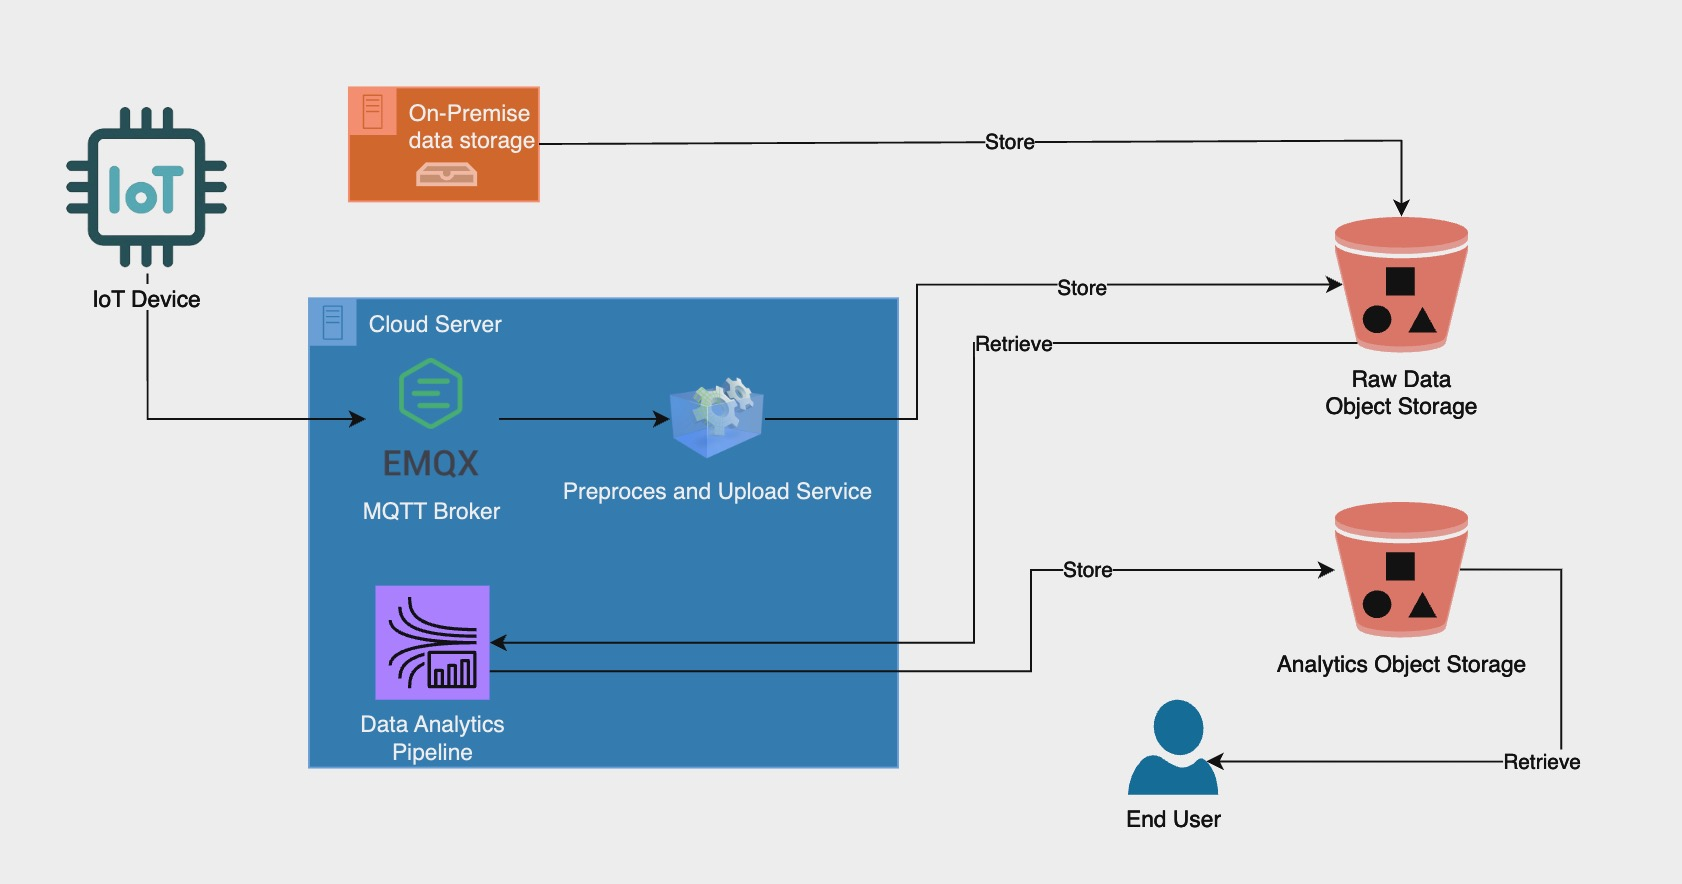
\includegraphics[width=1\textwidth]{Immagini/architecture.png}
    \caption{Architecture of the proposed solution}
    \label{fig:architecture}
\end{figure}

The architecture schematized in figure \ref{fig:architecture} is based on a modular, microservices approach. It is divided into three key layers: the data collection layer, the data storage layer, and the data analysis layer. Each layer addresses specific aspects of IoT data management, ensuring scalability, flexibility, and cloud-agnostic capabilities. The architecture is designed to handle large volumes of data from IoT devices and archive data sources.

\section{Data collection layer}

The data collection layer is responsible for ingesting data from various IoT devices and data archived on on-premise systems. This layer must support real-time data ingestion from IoT devices, as well as batch uploads of historical data.

\subsection{Data collection from IoT devices}
IoT devices send data to a cloud-hosted MQTT broker using the MQTT protocol, which is suitable for environments with limited bandwidth and high latency. Each IoT device publishes its data under specific MQTT topics, allowing for organized and efficient data routing. The collected data is structured in JSON format and contains timestamps and sensor readings. Before storage, the data is converted to CSV format for easier processing and analysis.

\subsection{Data collection from archived data}
The system also handles historical data uploads from on-premise sources. A simple script is used to upload archived CSV files to the cloud via the cloud provider's API. The data does not require preprocessing and is stored directly in object storage, making it available for further analysis.

\section{Data storage layer}

The data storage layer is designed to store both raw and analyzed data, using object storage as the primary storage solution. Object storage offers scalability, durability, and global accessibility, which makes it ideal for IoT data management. The architecture separates the storage of raw data from analyzed data by using different storage buckets, simplifying data management and ensuring efficient access to data for analysis.

This storage layer is inherently cloud-agnostic, as all major cloud providers offer similar object storage services. The solution can be deployed on any cloud provider with minimal adjustments, ensuring flexibility and avoiding vendor lock-in.

\section{Data analysis layer}

The data analysis layer retrieves preprocessed data from object storage for further processing and analysis. This layer supports a range of analytics operations, from simple statistical analysis to advanced machine learning and deep learning models. Data is first downloaded from the object storage to a local compute instance, as direct access to object storage file contents is not supported by cloud platforms.

Once the data is processed, the results are uploaded back to object storage in a separate bucket for easy access by other services or users. Data analysis can be triggered either automatically when new data is uploaded or manually via an API, depending on the specific requirements of the system.

\section{Cloud server (IaaS) vs. SaaS solutions}

The architecture makes use of Infrastructure as a Service (IaaS) to host the MQTT broker and the data analytics pipeline. While Software as a Service (SaaS) solutions offer convenience, the flexibility provided by IaaS allows for more control over the infrastructure and supports custom configurations and dependencies needed for the data analytics pipeline.

This approach also ensures that the system remains cloud-agnostic. Since all major cloud providers offer IaaS services, the architecture can be deployed on any platform without requiring significant modifications. Additionally, using IaaS gives the system better cost control over time, as pricing can be optimized based on the specific needs of the workload.

\section{Why the Proposed Architecture is Scalable}

Scalability is a core feature of the proposed architecture, allowing it to handle increasing volumes of data and expanding workloads without significant changes to the underlying structure. The system achieves scalability through several design principles:

\begin{itemize}
    \item \textbf{Microservices Architecture}: The architecture follows a microservices-based design, where different components (such as data collection, storage, and analysis) are loosely coupled and operate independently. This allows each service to be scaled independently based on the workload it handles. For example, the data analysis service can be scaled up to handle more intensive computations, while the data storage service can be scaled based on the amount of incoming data.
    
    \item \textbf{Horizontal and Vertical Scaling}: The architecture supports both horizontal scaling (adding more servers or instances to distribute the load) and vertical scaling (increasing the resources of existing servers). In the case of IoT data, which can grow exponentially, horizontal scaling is particularly valuable. For instance, additional computing servers can be added as the number of connected IoT devices increases. 
    
    \item \textbf{Cloud Infrastructure}: By utilizing cloud services such as Infrastructure as a Service (IaaS) and Object Storage, the architecture can leverage the inherent scalability of cloud platforms. Cloud providers offer auto-scaling features, enabling the system to automatically adjust resource allocation based on demand. This ensures that the architecture can handle variable workloads without manual intervention.

    \item \textbf{Object Storage}: The use of object storage allows the system to scale storage capacity without the need for complex infrastructure changes. Object storage systems are designed to handle vast amounts of unstructured data, making them ideal for IoT environments where data volume can increase rapidly. Since object storage scales automatically with the amount of data, the system can store large volumes of raw and processed data without performance degradation.
    
    \item \textbf{Distributed Data Processing}: The data analysis layer supports distributed data processing, allowing the workload to be spread across multiple servers or instances. This makes it possible to handle large-scale analytics tasks efficiently. Distributed processing frameworks such as Apache Spark could be integrated to perform parallel processing of large datasets, enhancing the system’s capacity to handle intensive computational tasks.

    \item \textbf{Event-Driven Architecture}: The system's event-driven design, particularly in the data collection and analysis layers, enables automatic scaling based on real-time data flow. When new data arrives, events can trigger scaling actions, such as adding more compute resources for analysis, ensuring that the system remains responsive even under high demand.
\end{itemize}

Overall, the architecture’s design ensures that it can scale in response to both growing data volumes and increased computational demands, making it suitable for a wide range of IoT applications. This scalability, combined with its cloud-agnostic nature, ensures that the system can grow and adapt without significant redesigns or performance trade-offs.


\section{Why the proposed architecture is cloud-agnostic}

The proposed architecture is designed to operate seamlessly on any cloud platform by leveraging standardized services and protocols. Key elements that make this architecture cloud-agnostic include:

\begin{itemize}
    \item \textbf{Object Storage}: The data storage layer uses object storage for both raw and processed data. Object storage services are available across all major cloud platforms, ensuring seamless integration with any provider.
    \item \textbf{MQTT Protocol}: The data collection layer uses MQTT, a lightweight messaging protocol widely supported by different cloud providers. This ensures flexibility and compatibility with various cloud-hosted or self-hosted MQTT brokers.
    \item \textbf{IaaS Services}: The use of IaaS to host the broker and data analysis services makes the system platform-independent. Any cloud provider that supports IaaS can host the solution without changes to the architecture.
\end{itemize}

By designing the system to use standardized components and protocols, the architecture ensures that the solution can be deployed on any cloud provider, reducing the risk of vendor lock-in and enhancing the ability to scale and adapt to different environments.

    \cleardoublepage
    \chapter{Test Implementation}
\label{cap:real_implementation}

To validate the proposed architecture and demonstrate its practical application, a real-world problem was selected for a proof of concept (PoC) implementation. Testing the architecture in a real-world scenario ensures that the system can meet the demands and challenges faced by actual users. In this PoC, however, actual users were simulated using MQTT clients to replicate the data upload patterns and volume expected in a real-world deployment. This approach highlights the scalability, reliability, and cloud-agnostic capabilities of the architecture when handling diverse workloads, making it an essential step for proving the viability of the solution.

The selected real-world problem comes from a company specializing in high-performance protective gear and technical apparel for motorsports and action sports. This case study aimed to develop a system that could analyze data from Inertial Measurement Units (IMUs) embedded in riders’ suits, providing feedback on performance, safety metrics, and crash detection. The client intends to use this system for both private users and professional motorsport pilots to improve riding performance and ensure safety.

Given the sporadic and intensive data generated by different types of users, the system needed to handle diverse upload patterns, manage a large volume of data, and provide insights in critical cases (such as detecting a crash). Testing the architecture in this context provides crucial feedback on the system’s ability to scale, manage data efficiently, and provide data analysis across different cloud platforms, such as Aruba Cloud and Azure.

\section{Why testing the architecture on a real-world problem?}
\label{sec:real_world_problem}

Implementing the architecture in a real-world scenario provides several benefits beyond theoretical testing:
\begin{itemize}
    \item \textbf{Scalability Testing}: Since users upload varying amounts of data based on actual usage patterns, this helps validate the system’s ability to scale both horizontally and vertically.
    \item \textbf{Performance and Resource Utilization}: The architecture’s ability to manage the load under real conditions, such as spikes in data uploads, can be accurately measured, enabling optimization of resource utilization.
    \item \textbf{Cloud-Agnostic Validation}: Testing across multiple cloud providers (in this case, Aruba Cloud and Azure) proves that the architecture can operate without significant modification, reducing vendor lock-in.
    \item \textbf{User Interaction and Feedback}: Real-world testing provides insights into how users would interact with the system, enabling further refinement of the user experience and data handling mechanisms.
\end{itemize}

By addressing these aspects, the PoC implementation of the system offers a comprehensive assessment of the architecture’s practical performance and highlights potential areas for improvement, ensuring that it can support future real-world deployments.

\section{Implementation of the data collection layer}
\label{sec:implementation_data_collection}

The data collection layer is responsible for gathering data from the biker suits and uploading it to cloud storage for further processing. This layer handles two key tasks: MQTT data ingestion from the IMUs and uploading archived data.

\subsection{Data ingestion from MQTT}
To handle MQTT data ingestion, the system uses an MQTT broker, specifically the EMQX broker, which was selected for its scalability and cloud-agnostic nature. The MQTT broker receives data from the IMUs in JSON format, which is published to specific MQTT topics based on the type of data and the user.

In the PoC, the IMUs were simulated using the MQTTX tool to emulate data from the biker suits. Each device published JSON messages containing timestamps and sensor data (such as acceleration and gyroscope readings). The MQTT broker was configured on both Aruba Cloud and Azure servers to validate the cloud-agnostic nature of the architecture.

\textbf{Implementation Details}:
\begin{itemize}
    \item \textbf{MQTT Topics}: Each biker suit publishes data to its own MQTT topic, allowing easy organization and routing of messages.
    \item \textbf{Broker Testing}: The broker was tested by simulating data uploads using MQTTX clients. The system successfully received the data, confirming the stability and scalability of the MQTT broker.
\end{itemize}

\subsubsection{Preprocessing pipeline}
After receiving data from the MQTT broker, the next step in the data collection layer is the preprocessing pipeline, which converts the incoming JSON data into a CSV format for easier processing and storage. The pipeline was implemented using a Python script that subscribes to the MQTT broker, parses the JSON data, and stores it locally. The code of the script is provided in Section \ref{sec:prprocessing_impl}. Sucessively, another script uploads the data to the object storage, and its code is provided in Section \ref{sec:upload_cloudcloud_impl}.

\textbf{Implementation Details}:
\begin{itemize}
    \item \textbf{Data Parsing}: The pipeline extracts timestamps and sensor values from the JSON messages, converts them into CSV rows, and stores them in object storage.
    \item \textbf{Cloud-Agnostic Storage}: The CSV files were uploaded to object storage on both Azure Blob Storage and Aruba Cloud, proving that the preprocessing pipeline works across different cloud platforms.
\end{itemize}

\subsection{Data ingestion from archived data}
\label{sec:archived_data_ingestion}

In addition to the MQTT-based data ingestion from IoT devices, the system must also support the ingestion of archived data, typically collected and stored locally. This archived data needs to be uploaded to cloud storage for further processing and analysis. The ingestion of archived data ensures that both historical and MQTT-ingested data can be integrated into the system seamlessly, providing a comprehensive view of the dataset for users and allowing retrospective analyses.

In this implementation, archived data is expected to be stored locally in CSV format. A Python script is used to upload this archived data from an on-premise location to the cloud object storage, where it can be accessed by the data analysis pipeline. The script handles large batch uploads and is designed to operate across different cloud environments (such as Azure Blob Storage and Aruba Cloud Object Storage), maintaining the cloud-agnostic nature of the system. The code for the implementation is provided in Section \ref{sec:upload_cloudcloud_impl}.

\textbf{Implementation Details}:
\begin{itemize}
    \item \textbf{File Structure}: The archived data is expected to follow a structured format (e.g., CSV) that is compatible with the analysis pipelines.
    \item \textbf{Upload Mechanism}: The script leverages the cloud provider's API to handle file uploads, ensuring compatibility with various storage providers.
    \item \textbf{Batch Processing}: The system supports bulk uploads of multiple files, making it efficient for handling large datasets. The script can upload entire directories or specific files as needed.
    \item \textbf{Storage Confirmation}: After each file is uploaded, the system verifies its successful transfer to the cloud storage and logs any failures for troubleshooting.
\end{itemize}

\section{Implementation of the data storage layer}
\label{sec:implementation_data_storage}

The data storage layer handles the storage of both raw and processed data in cloud object storage. Object storage was chosen for its scalability and flexibility, allowing the system to manage large volumes of unstructured data efficiently.

\subsection{Object storage configuration}
In the PoC, object storage was set up on both Azure and Aruba Cloud. Separate storage buckets were created to manage raw data, processed analytics, and crash-specific data. The separation of data ensures that raw sensor data can be archived, while processed data is readily accessible for further analysis or user requests. An example of data stored on Aruba Object Storage and Azure Blob Storage can be seen respectively in Figure \ref{fig:aruba_obj_storage} and \ref{fig:azure_obj_storage}.

\textbf{Implementation Details}:
\begin{itemize}
    \item \textbf{Raw Data Storage}: Data from the biker suits was uploaded to raw data buckets in both Azure and Aruba Cloud Object Storage.
    \item \textbf{Processed Data Storage}: The data analysis component stores results in separate analytics buckets, while crash-specific data is stored in dedicated buckets.
    \item \textbf{Testing}: The storage layer was tested by uploading and retrieving both raw and processed data from the cloud storage services, demonstrating the cloud-agnostic nature of the system.
\end{itemize}

\begin{figure}[htbp]
    \centering
    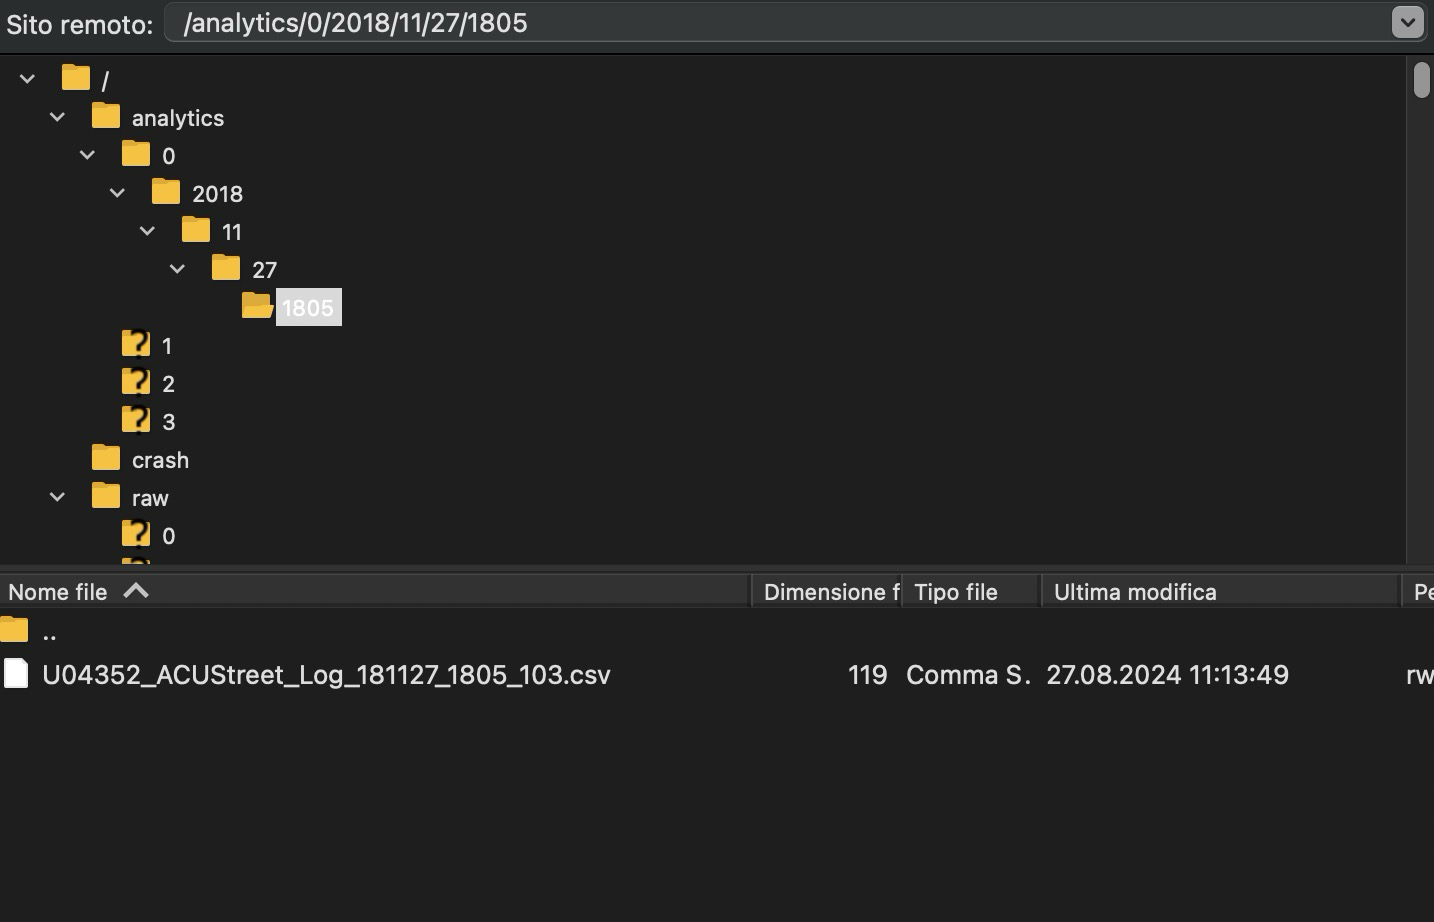
\includegraphics[width=1\textwidth]{Immagini/data_storage.png}
    \caption{Example of data stored on Aruba Object Storage}
    \label{fig:aruba_obj_storage}
\end{figure}

\begin{figure}[htbp]
    \centering
    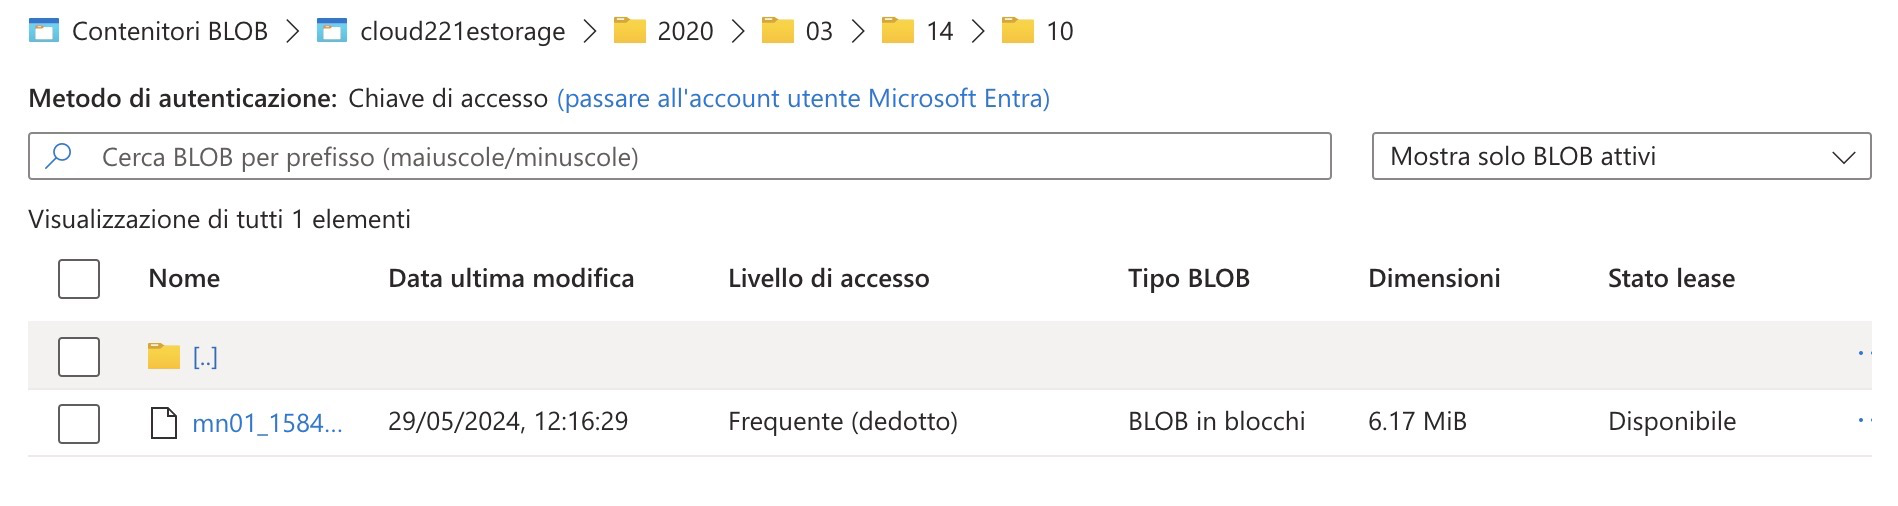
\includegraphics[width=1\textwidth]{Immagini/azure_storage.png}
    \caption{Example of data stored on Azure Blob Storage}
    \label{fig:azure_obj_storage}
\end{figure}


\section{Implementation of the data analysis layer}
\label{sec:implementation_data_analysis}

The data analysis layer is responsible for processing the collected data, running analytics, and storing the results. In this implementation, the data analysis layer retrieves preprocessed data, performs the required analysis, and stores the results back in object storage.

\subsection{Data processing pipeline}
\label{sec:data_processing_pipeline}

The data processing pipeline was implemented using Java. The pipeline reads and processes the preprocessed CSV data stored in object storage. The pipeline performs essential tasks such as calculating average speed, detecting left and right turns, identifying maximum acceleration and deceleration, and flagging potential crash events based on sensor data.

\textbf{Implementation Details}:
\begin{itemize}
    \item \textbf{CSV Data Processing}: The Java function reads the sensor data from a CSV file, processes key metrics such as speed, acceleration, and orientation, and calculates values like the highest acceleration, deceleration, and average speed.
    \item \textbf{Turn Detection}: Left and right turns are detected based on changes in the orientation angle of the rider, derived from chest orientation sensor data. 
    \item \textbf{Storage of Results}: After processing, the calculated metrics are stored in a structured format (e.g., a map) for later storage or further analysis.
\end{itemize}

The processing pipeline reads the CSV data using Apache Commons CSV, a library that simplifies reading and parsing CSV files. The script processes each record, extracting relevant sensor data, performing calculations, and storing the resulting metrics in a key-value format for further use. The following metrics are calculated: highest acceleration, highest deceleration, average speed, and the number of left and right turns.

For more details on the implementation of the data processing function, refer to the code in Section \ref{sec:analysis_fun}, while an example of the result of the analysis process can be seen in figure \ref{fig:analysis}.
\begin{figure}[htbp]
    \centering
    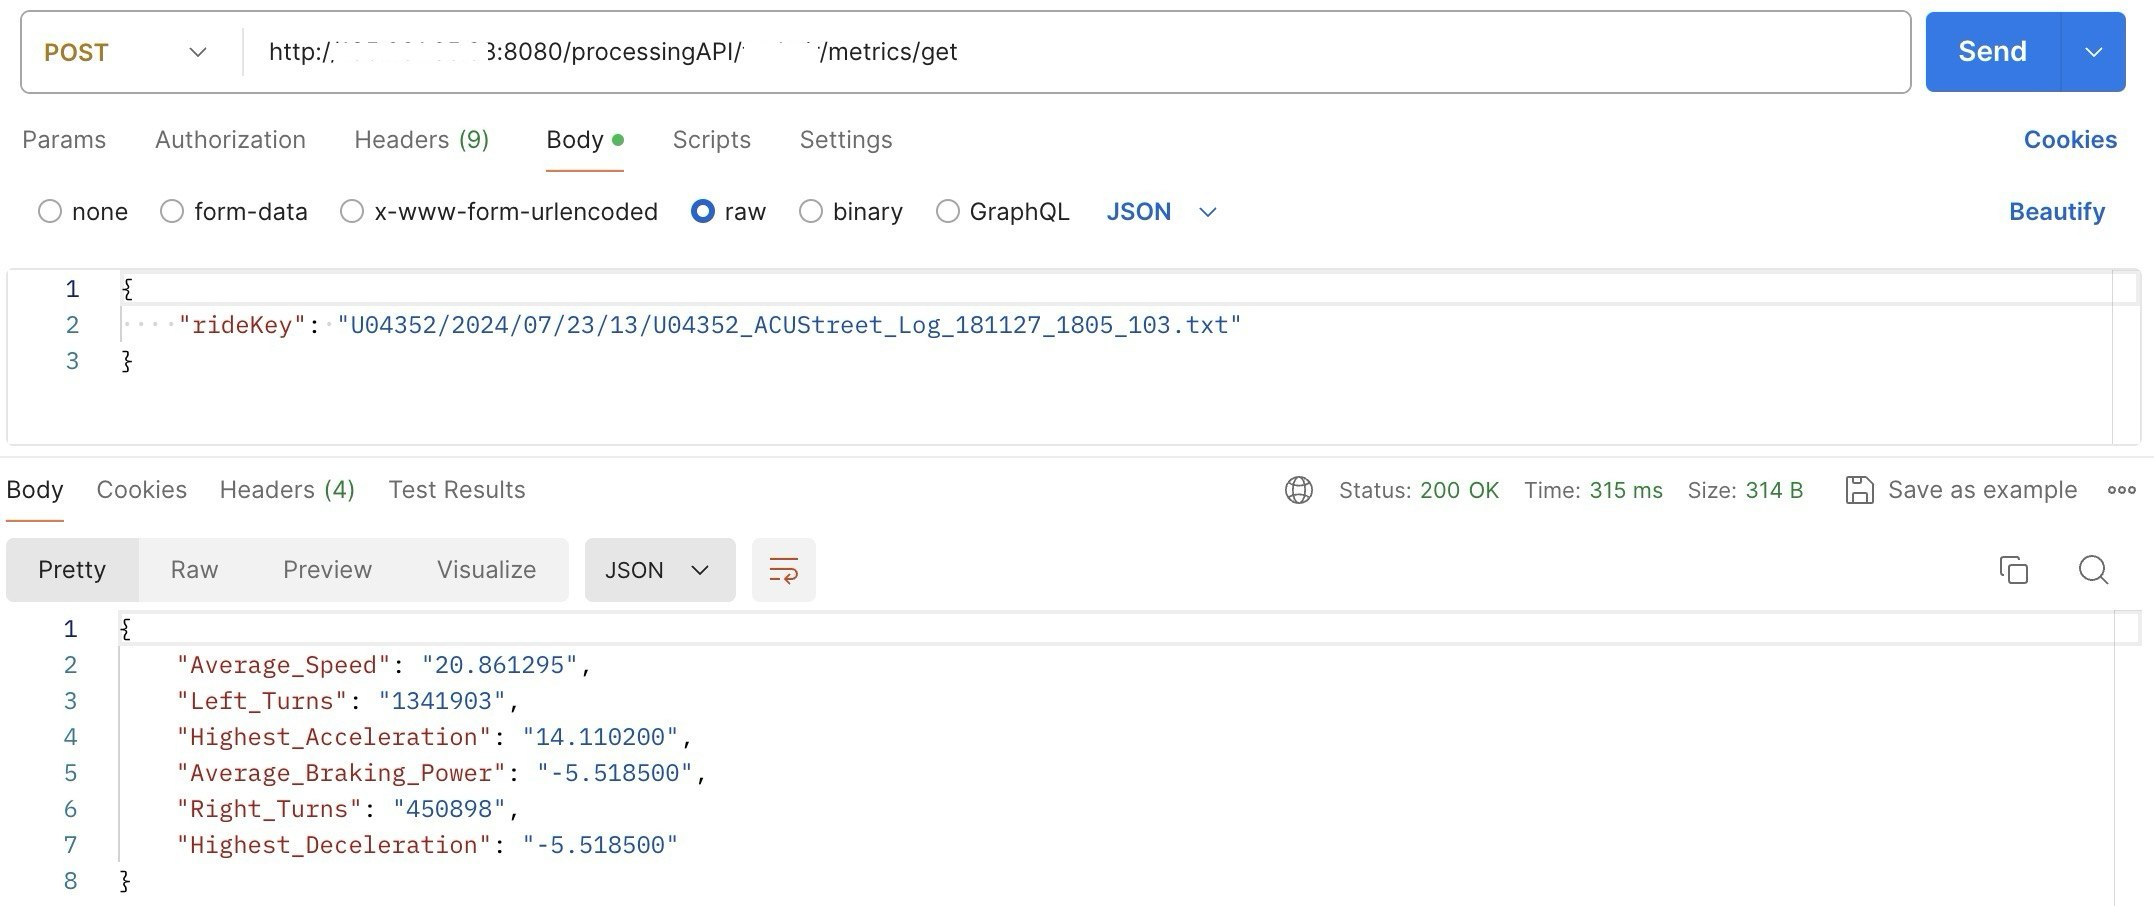
\includegraphics[width=1\textwidth]{Immagini/get_metrics.png}
    \caption{Example of results of the analysis process}
    \label{fig:analysis}
\end{figure}

    \cleardoublepage
    \chapter{Testing}
\label{cap:testing}

After implementing the system, a series of tests were conducted to ensure it met the client’s requirements and performed as expected. The testing phase included various types of tests such as unit, integration, and performance testing to validate the system’s functionality, reliability, and scalability under real-world conditions.

The tests were conducted on a machine with limited resources, without enabling scaling, to evaluate the system’s performance in a worst-case scenario. This approach allowed for the identification of potential bottlenecks and performance issues under constrained environments, providing valuable insights into the system's baseline performance and areas for optimization.

\section{Unit testing}
Unit tests were conducted to verify the functionality of individual components like upload scripts, data ingestion, and data processing functions. Although manual unit tests were performed in this phase, they helped isolate each component to ensure it functioned as expected and produced the correct output. A more comprehensive automated unit testing framework will be implemented in future phases to ensure continuous validation.

\section{Integration testing}
Integration tests were conducted to validate the interactions between various components, including the data ingestion, storage, and processing pipelines. These tests ensured that the components worked seamlessly together, processing and storing data accurately. The integration tests were carried out in an environment replicating the production setup, ensuring that the system would behave correctly in a real-world scenario. While these tests were conducted manually, an automated integration testing framework will be implemented in future iterations to streamline the testing process.

\section{Performance testing}
Performance tests were conducted to evaluate the system’s scalability, reliability, and responsiveness under varying load conditions. These tests aimed to measure throughput, latency, and resource utilization to identify potential bottlenecks. 

For these tests, the system was run on a machine with limited resources, and scaling was not enabled to assess how the system would perform under constrained conditions. This approach was selected to test the system in a worst-case scenario, allowing us to observe its performance under maximum stress and ensure that it could handle significant workloads even without the benefits of resource scaling.

The following tests were performed on a single server with a subset of users. Further testing in a distributed environment, with multiple servers, will be conducted in the next phase to evaluate system performance in a more complex setup.

\section{Stress test results}
The results of the stress tests are summarized in Table \ref{table:performance_metrics}. These tests focused on two key operations: calculating analytics and retrieving analytics.

\begin{table}[htbp]
\centering
\begin{tabular}{|c|c|c|}
\hline
\textbf{Number of Users} & \textbf{Calculate Analytics} & \textbf{Retrieve Analytics} \\
\hline
1   & 30 sec              & 221 ms          \\
\hline
10  & 85 sec (1 min 25 sec)& 252 ms          \\
\hline
50  & 467 sec (7 min 47 sec)& 327 ms          \\
\hline
250 & 2284 sec (38 min 4 sec)& 268 ms          \\
\hline
\end{tabular}
\caption{Performance Metrics for Calculating and Retrieving Analytics}
\label{table:performance_metrics}
\end{table}

\subsection{Analysis of results}
The performance metrics in Table \ref{table:performance_metrics} indicate how the system handled different numbers of concurrent users for the two operations:

\begin{itemize}
    \item \textbf{Calculate Analytics}:
        \begin{itemize}
            \item With 1 user, the operation took 30 seconds.
            \item As the number of users increased to 10, the time rose to 85 seconds.
            \item With 50 users, the time increased drastically to 467 seconds.
            \item At 250 users, the operation took 2284 seconds (38 minutes and 4 seconds).
            \item This significant increase in time suggests a bottleneck, primarily due to the large volume of data being transferred from object storage to the analytics pipeline on the server. The performance bottleneck is more pronounced due to the limited resources available, simulating a worst-case scenario.
        \end{itemize}

    \item \textbf{Retrieve Analytics}:
        \begin{itemize}
            \item The response time remained relatively stable, ranging from 221 ms to 327 ms as the number of users increased from 1 to 250.
            \item The minor variations in response time indicate that the system efficiently handled retrieval operations, even with high concurrent loads, despite the machine's limited resources.
        \end{itemize}
\end{itemize}

\section{Conclusions}
The performance tests highlight that while the system handles retrieval efficiently under increasing loads, calculating analytics experiences significant performance degradation as the number of concurrent users rises. The bottleneck is mainly due to the high volume of data transferred from object storage to the analytics pipeline, exacerbated by the resource limitations of the test environment.

\textbf{Next steps for optimization}:
\begin{itemize}
    \item \textbf{Horizontal Scaling}: The system could be scaled horizontally by distributing the workload across more servers. This would reduce the load on individual servers and improve processing times.
    \item \textbf{Optimizing Data Transfer}: Saving raw data directly on the server could improve performance, but it would require more storage and may not be scalable. Another solution is to optimize the data transfer process between object storage and the server.
    \item \textbf{Containerization}: Deploying the application in a containerized environment, such as Kubernetes, could help distribute the load more efficiently across multiple servers. This approach would enable the system to scale horizontally as needed and improve performance under heavy loads.
\end{itemize}

By testing under constrained resources and without scaling, we could identify the system’s worst-case performance, providing valuable insights into potential bottlenecks. This testing approach has demonstrated that, while the system is capable of handling up to 250 concurrent users, optimizations and scaling mechanisms will be necessary to support larger user bases and more demanding real-world conditions.

    \cleardoublepage
      \chapter{Conclusion}
\label{cap:conclusion}

In this chapter, the conclusions of the work are presented. The objectives achieved are discussed, as well as the future developments of the project. The author also reflects on the learnings gained during the project’s development.

\section{Objectives achieved}

The main goal of this project was to design and implement a scalable, cloud-agnostic architecture capable of ingesting data from multiple sources, processing it, and storing it in a data lake. This objective was successfully achieved through the engineering, development, and testing of the architecture, as described in Chapter \ref{cap:method}. The system was tested on both Aruba Cloud and Microsoft Azure to assess its cloud-agnostic nature, confirming its capability to function seamlessly across different cloud platforms.

The architecture was validated through a real-world implementation, which demonstrated its flexibility and scalability (Chapter \ref{cap:real_implementation}). The system was capable of ingesting data, processing analytics, and handling large volumes of information in a cloud-agnostic manner, ensuring that the architecture could scale effectively to meet real-world demands. Security constraints were also addressed using the shared responsibility model of the cloud providers, and encryption was implemented both at rest and in transit.

\section{Future developments}

The future development of this project can focus primarily on enhancing the base architecture. The Proof of Concept (PoC) was designed to validate its capabilities, and moving forward, there are several areas for improvement and extension that can solidify the architecture’s scalability, flexibility, and cloud-agnostic nature.

\subsection{Architecture enhancements}
To further strengthen the base architecture, the following advancements are recommended:

\begin{itemize}
    \item \textbf{Edge Computing Integration}: Incorporating edge computing capabilities into the architecture would significantly reduce latency and improve real-time processing. This can be achieved by training machine learning models in the cloud and deploying them on edge devices. With this approach, data can be processed closer to its source, minimizing the need for constant communication with the cloud and allowing for faster decision-making, which is especially valuable for time-sensitive applications like IoT and autonomous systems.
    
    \item \textbf{Wider Cloud Provider Testing}: While the current implementation demonstrated the architecture’s cloud-agnostic capabilities across Aruba Cloud and Azure, future testing should expand to include other major cloud platforms such as AWS, Google Cloud, and Oracle Cloud. This will help validate that the architecture can seamlessly adapt to different environments without major modifications, ensuring compatibility across a broader range of platforms and reducing the risk of vendor lock-in.

    \item \textbf{Enhanced Security and Compliance}: As the architecture grows in complexity and scale, incorporating advanced security features will be essential. This includes integrating role-based access control (RBAC), multi-factor authentication (MFA), and enhanced encryption standards. Additionally, ensuring compliance with industry regulations such as GDPR, HIPAA, and SOC2 will become increasingly important as the system scales and handles more sensitive data.

    \item \textbf{Performance Optimization}: Optimizing the performance of the data processing pipeline, particularly for handling high volumes of concurrent requests, should be a key focus. This can involve fine-tuning data transfer mechanisms, improving parallel processing capabilities, and leveraging distributed computing techniques. Additionally, containerizing the application using platforms like Kubernetes would improve scalability and resource management, allowing the architecture to handle larger workloads efficiently.

    \item \textbf{Comprehensive Testing Framework}: Introducing an automated testing framework for unit, integration, and performance testing will help ensure that future developments are thoroughly validated before deployment. Automated testing will streamline the development cycle, making it easier to detect and resolve issues early while maintaining system stability.
\end{itemize}

\section{Final thoughts}

The development of a scalable, cloud-agnostic architecture provided valuable insights into cloud computing, data ingestion, and real-time processing. The PoC tested the architecture's flexibility, reliability, and scalability across multiple platforms, laying the groundwork for future enhancements. By focusing on edge computing, further cloud-agnostic testing, and performance optimization, this architecture has the potential to support a wide range of use cases beyond its initial scope.

Building adaptable solutions that are cloud-agnostic ensures the architecture’s long-term sustainability and allows it to evolve with industry needs. As organizations increasingly require scalable, secure, and flexible cloud architectures, this project provides a robust foundation for meeting those demands across diverse applications and environments.

    \cleardoublepage
    \appendix
\chapter{Code listings}
\label{appendix:code}

This appendix contains the key code components used in the Proof of Concept (PoC) implementation. Each section corresponds to a specific layer or component of the architecture described in Chapter \ref{cap:real_implementation}. The code is divided into sections based on the data pipeline: from ingestion to storage and data analysis.

\section{Preprocessing pipeline}
\label{sec:prprocessing_impl}

The following script subscribes to the MQTT broker and processes incoming messages from the IoT devices. The script converts JSON data into CSV format for easier storage and further processing.

\textbf{Explanation:}  
- The script connects to the MQTT broker and listens for messages from IoT devices.  
- Upon receiving a message, the script extracts sensor data from the JSON payload and writes it into a CSV file.  
- The file is saved locally before being uploaded to cloud storage.

\begin{verbatim}
#!/root/y/bin/python3
import paho.mqtt.client as mqtt
import datetime
import os
import json
import csv
import sys
sys.stdout = open('logs.txt', 'w')
sys.stderr = sys.stdout

def json_to_csv(value):
    """
    Converts a JSON object to a CSV string.
    
    Args:
        value (dict): The JSON object to be converted.
    
    Returns:
        str: The CSV string representation of the JSON object.
    """
    csv_data = []
    
    # Extracting headers from the first object in the JSON
    headers = list(value.keys())
    
    # Adding headers to the CSV
    csv_data.append(headers)
    
    # Adding values to the CSV
    csv_data.append([value[header] for header in headers])

    return csv_data

# Message receiving callback
def on_message(client, userdata, msg):
    _id = msg.topic.split('/')[-1]
    filename = _id + '_' + str(datetime.datetime.now().strftime('%Y-%m-%dH%H')) + '.csv'
    filepath= "/root/CloudUtils/ToUpload"
    data = json.loads(msg.payload.decode())
    properties = data['SystemProperties']
    data = data['Body']
    csv_data = json_to_csv(data)
    if not os.path.exists(filepath):
        os.makedirs(filepath)
    filepath = os.path.join(filepath, filename)
    if os.path.exists(filepath):
        csv_data = csv_data[1:]
    else:
        csv_data.insert(0, ['SystemProperties: ' + str(properties)])
    try:
        with open(filepath, 'a') as file:
            writer = csv.writer(file, delimiter='\t')
            writer.writerows(csv_data)
    except FileNotFoundError:
       pass

#Connection callbacks
def on_connect(client, userdata, flags, rc):
    print('Connected with result code '+str(rc))
    client.subscribe('221e/#')

def on_disconnect(client, userdata, rc):
    print('Disconnected with result code '+str(rc))
    client.reconnect()

# Load application properties
with open('/root/CloudUtils/application_properties.json') as file:
    properties = json.load(file)
    username = properties['mqttx-username']
    password = properties['mqttx-password']
    ip = properties['mqttx-host']
    port = properties['mqttx-port']

client = mqtt.Client()
client.username_pw_set(username, password)
client.tls_set(ca_certs='/Certs/ca-root-cert.crt', certfile='/Certs/server.crt', keyfile='/Certs/server.key')
client.connect(ip, port, 0)

client.on_connect = on_connect
client.on_message = on_message
client.on_disconnect = on_disconnect

client.loop_forever()
\end{verbatim}

\section{Upload data to object storage}
\label{sec:upload_cloudcloud_impl}

This script uploads the locally saved CSV files from the preprocessing step to the cloud storage (S3-compatible services like Azure Blob Storage or Aruba Cloud).

\textbf{Explanation:}  
- The script iterates through the files in a specified directory and uploads them to the cloud storage bucket.  
- After successful uploads, the files are removed from the local system to optimize storage.

\begin{verbatim}
#!/root/y/bin/python3
import boto3
import os
import json
from datetime import datetime

# Configuration
endpoint_url = ''
access_key = ''  # Username equivalent
secret_key = ''  # Password equivalent
bucket_name = 'raw'
walk_dir = ''

with open('/root/CloudUtils/application_properties.json') as file:
    properties = json.load(file)
    endpoint_url = properties['s3_host']
    access_key = properties['s3_user']
    secret_key = properties['s3_pwd']
    walk_dir = properties['WalkDir']

# Create a session and client
session = boto3.session.Session()
s3 = session.client(
    's3',
    endpoint_url=endpoint_url,
    aws_access_key_id=access_key,
    aws_secret_access_key=secret_key
)

for subdir, dirs, files in os.walk(walk_dir):
    for file in files:
        path= subdir + '/' + file
        if file.startswith('.'):
            continue
        if os.stat(path).st_size == 0:
            continue

        # Extract device ID and timestamp
        _id = file.split('_')[0]
        timestamp = datetime.strptime(file.split('_')[1].split('.')[0], '%Y-%m-%dH%H')
        timestamp = datetime.timestamp(timestamp)
        timestamp = str(timestamp).split('.')[0]

        datet_time=file.split('_')[1].split('.')[0]
        date=datet_time.split('H')[0].split('-')
        time=datet_time.split('H')[1]
        key= _id+"/"+date[0]+"/"+ date[1] +"/"+ date[2]+"/"+time+"/"+file

        # Upload file to the cloud
        s3.upload_file(path, bucket_name, key)
        try:
            s3.head_object(Bucket=bucket_name, Key=key)
            os.remove(path)
        except:
            continue
\end{verbatim}

\section{Data analysis function}
\label{sec:analysis_fun}

This Java function reads the preprocessed CSV files and calculates performance metrics such as average speed, left/right turns, and acceleration/deceleration values.

\textbf{Explanation:}  
- The function processes each CSV file, iterating through the records to compute statistics like the highest acceleration and deceleration, average speed, and detecting left or right turns.  
- The calculated metrics are stored in a map for further analysis or storage.

\begin{verbatim}
/*
 * Process CSV
 * @param String filePath: file path
 * @return Map<String, Object>: map of metrics
 * */
private Map<String, Object> processCSV(String filePath) throws IOException {
    Map<String, Object> metrics = new HashMap<>();
    try (Reader reader = new FileReader(filePath);
         CSVParser csvParser = new CSVParser(reader,
            CSVFormat.DEFAULT.withDelimiter('\t').withFirstRecordAsHeader())) {

        double highestAcceleration = Double.MIN_VALUE;
        double highestDeceleration = Double.MAX_VALUE;
        double totalSpeed = 0;
        int speedCount = 0;
        int leftTurns = 0;
        int rightTurns = 0;

        for (CSVRecord record : csvParser) {
            double accelChestX = Double.parseDouble(record.get("Accel_CHEST.X"));
            double accelChestY = Double.parseDouble(record.get("Accel_CHEST.Y"));
            double accelChestZ = Double.parseDouble(record.get("Accel_CHEST.Z"));
            double gpsSpeed = Double.parseDouble(record.get("GPS_Speed."));

            highestAcceleration = Math.max(highestAcceleration, 
                Math.max(accelChestX, Math.max(accelChestY, accelChestZ)));
            highestDeceleration = Math.min(highestDeceleration,
                Math.min(accelChestX, Math.min(accelChestY, accelChestZ)));

            totalSpeed += gpsSpeed;
            speedCount++;

            double orientChestX = Double.parseDouble(record.get("Orient_CHEST.X"));
            double orientChestY = Double.parseDouble(record.get("Orient_CHEST.Y"));
            double orientationAngle = Math.atan2(orientChestY, orientChestX) * (180 / Math.PI);

            if (orientationAngle > 25) leftTurns++;
            if (orientationAngle < -25) rightTurns++;
        }

        double averageSpeed = totalSpeed / speedCount;

        metrics.put("Left_Turns", leftTurns);
        metrics.put("Right_Turns", rightTurns);
        metrics.put("Average_Speed", averageSpeed);
        metrics.put("Highest_Acceleration", highestAcceleration);
        metrics.put("Average_Braking_Power", highestDeceleration);
        metrics.put("Highest_Deceleration", highestDeceleration);
    }

    return metrics;
}
\end{verbatim}

    \cleardoublepage

    \printbibliography[heading=bibintoc]
\end{document}
